\section{The Gravity and Gravity-Inertia wave equations}\label{Chapter4}

In this chapter we consider the equations describing the horizontal
propagation of gravity and gravity-inertia waves. Mathematically, this
means that we will be dealing with a system of two or three partial
differential equa­tions of the first order. Thus, we will now have two
or three dependent variables. The system of equations will always be
equivalent to a single differential equation of a higher order. This
equation can be obtained from the system by elimination of dependent
variables.

We first put this problem in perspective. Arakawa, (Arakawa, 1970), has
stated that there are two main problems in finite difference
integrations of the atmo­spheric governing equations. One is a proper
simulation of the geostrophic adjustment process. Through this process
the atmosphere establishes a characteristic quasi-nondivergent state,
mostly as a result of the dispersion of the gravity-inertia waves. The
associated computa­tional considerations will be discussed in this
chapter. The second problem is the prediction or simulation of the
large-scale quasi-nondivergent flow after it has been established. Here
the horizontal advection is the dominat­ing mechanism. The associated
computational consi­derations were discussed in the preceding chapter.

Extensive study of the problems in integrations of the gravity-inertia
wave equations began in atmospheric modelling much later than studies of
the advection problem. After Richardson\textquotesingle s (1922) first
unsuccessful numerical integration of the complete primitive equa­tions,
the successful result of Charney, Fjortoft and von Neumann (1950) was
largely due to the exclusion of gravity-inertia waves from their
equations by using the geostrophic approximation in the vorticity
equation. The governing equations with the gravity-inertia waves
excluded, are customarily called the filtered equations. They bypass the
geostrophic adjustment problem. The filtered equations were used almost
exclusively in the first decade of numerical forecasting research.

Efforts to improve the performance of numerical models led to a desire
to include the non-geostrophic effects. This is very difficult to do
within the modified system of equations. Thus, starting with the first
success­ful experiments by Hinkelmann (1959), modellers came back to
using the primitive equations. Except for special purposes, the
primitive equations are used almost

exclusively in atmospheric models today. They are generally considered
superior for both research and operational applications (e.g. Sawyer,
1972). The speed of propagation of the gravity and gravity-inertia
waves, and their sensitivity to various numerical errors mean that their
treatment requires especially careful consideration.

\subsection{\texorpdfstring{\textbf{One-dimensional gravity waves:
centered space
differencing}}{One-dimensional gravity waves: centered space differencing}}\label{one-dimensional-gravity-waves-centered-space-differencing}

We shall first consider the simplest case of gravity waves where the
dependent variables are functions of one space variable. They are
governed by the linearized equations

{\[\frac{\partial u}{\partial t} &= - g\frac{\partial h}{\partial x}\]\[\frac{\partial h}{\partial t} &= - H\frac{\partial u}{\partial x},\]\[&g,H = \text{const}\]}

Thus, we have a system with two dependent and two independent variables.

We seek wave solutions of \texttt{b1.1} in the form

{\[u(x,t) = \text{Re} \left[ \widehat{u} e^{i(k x - \nu t)} \right]\]\[h(x,t) = \text{Re} \left[ \widehat{h} e^{i(k x - \nu t)} \right]\]}

and obtain the homogeneous system

\[v\widehat{u} &= gk\widehat{h}\]\[v\widehat{h} &= Hk\widehat{u}\]

giving the frequency equation

{\[v^{2} =gH k^{2}\]}

Thus,

{\[c = \frac{v}{k} = \pm \sqrt{gH}\]}

showing that the gravity waves can propagate along the \emph{x} axis in
both directions at a speed \(\sqrt{gH}\). This speed is not a function
of wave number so that there is no dispersion of the waves.

Consider now the differential-difference equations

{\[\frac{\partial u_{j}}{\partial t} &= - g\frac{h_{j + 1} - h_{j - 1}}{2\Delta x}\]\[\frac{\partial h_{j}}{\partial t} &= - H\frac{u_{j + 1} - u_{j - 1}}{2\Delta x}\]}

that we obtain when the space derivatives in \texttt{b1.1} are
approximated by centered finite difference quotients using values at the
two nearest points. The solutions \texttt{b1.2} now take the form

{\[u_{j}\left( t \right) = Re\left\lbrack \widehat{u}e^{i\left( kj\Delta x - vt \right)} \right\rbrack\]\[h_{j}\left( t \right) = Re\left\lbrack \widehat{h}e^{i\left( kj\Delta x - vt \right)} \right\rbrack\]}

Substitution of these solutions into \texttt{b1.5} leads to

\[\nu\widehat{u} = g\frac{\sin{k\Delta x}}{\Delta x}\widehat{h}\]\[\nu\widehat{h} = H\frac{\sin{k\Delta x}}{\Delta x}\widehat{u}\]

giving the frequency equation

{\[\nu^{2} = gH\left( \frac{\sin{k\Delta x}}{\Delta x} \right)^{2}\]}

Thus, instead of a constant phase speed, the gravity waves now propagate
with the phase speed

{\[c^{*} = \pm \sqrt{gH}\frac{\sin{k\Delta x}}{k \Delta x}\]}

or

{\[c^{*} = c \frac{\sin{k\Delta x}}{k\Delta x}\]}

This phase speed is a function of wave number, and, thus, we see that
the space differencing again results in compu­tational dispersion. The
formula \texttt{b1.9} is the same as the one obtained in the preceding
chapter when consider­ing the advection equation. Therefore, both the
phase speed and the group velocity depend on the wave number as shown in
\texttt{figg:14} of the preceding chapter. The phase speed decreases as
the wave length decreases, and the wave with wave length \(2\Delta x\)
is stationary.

There is, however, an important difference between this problem and the
advection problem because we now have two dependent variables. We have
assumed that they are both carried at every grid point, as shown in
\texttt{figg:411}

\begin{figure}
\centering
\pandocbounded{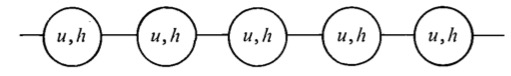
\includegraphics[keepaspectratio]{./pictest/pic411.jpg}}
\caption{}
\end{figure}

As far as the system \texttt{b1.5} is concerned, however, the underlined
variables in the figure depend only on other underlined variables. The
same statement holds for the variables that are not underlined. Thus,
the grid in the figure contains two elementary "subgrids", with the
solution on one of these subgrids being completely decoupled from the
other. Thus, it would be better to calculate only one of these
solutions, that is, to use a grid as shown in \texttt{figg:412}. Such a
grid, with variables carried at alternate points in space, is called a
\emph{staggered grid}. The computation time needed to solve
\texttt{b1.5} on the grid is reduced by a factor of two, and the
truncation error is the same. Furthermore, the waves with
\(k\Delta x > \frac{\pi}{2}\) have been eliminated, and these are just
the waves associated with large phase speed errors and negative group
velocities.

\begin{figure}
\centering
\pandocbounded{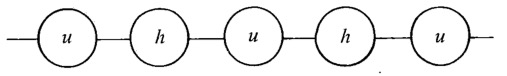
\includegraphics[keepaspectratio]{./pictest/pic412.jpg}}
\caption{}
\end{figure}

Thus, when using such a staggered grid, the phase speed and group
velocity diagram shown in \texttt{figg:14} of the preceding chapter is
reduced to its left half, covering waves with wave lengths of up to
\(4\Delta x\) only. This is a tremendous improvement.

If we wish to have waves with wave lengths between \(4\Delta x\) and
\(2\Delta x\) in our calculation we can reduce the grid length by a
factor of two and perform a much more accurate integration, using the
same amount of compu­tation time than with a grid that is not staggered.

\subsection{\texorpdfstring{\textbf{Two-dimensional gravity
waves}}{Two-dimensional gravity waves}}\label{Section4.2}

We now consider \emph{two-dimensional} gravity waves. Thus, we consider
the system of linearized equations

{\[\frac{\partial u}{\partial t} &= - g\frac{\partial h}{\partial x}\]\[\frac{\partial v}{\partial t} &= - g\frac{\partial h}{\partial y}\]\[\frac{\partial h}{\partial t} &= - H\nabla\cdot\textbf{v}\]}

Substituting the wave solutions

{\[u = Re\left\lbrack \widehat{u}e^{i\left( kx + ly - \nu t \right)} \right\rbrack\]\[v = Re\left\lbrack \widehat{v}e^{i\left( kx + ly - \nu t \right)} \right\rbrack\]\[h = Re\left\lbrack \widehat{h}e^{i\left( kx + ly - \nu t \right)} \right\rbrack\]}

We now obtain

{\[\nu^{2} = gH\left( k^{2} + l^{2} \right)\]}

Thus, in the two-dimensional case, the gravity waves propagate with the
same constant phase speed \(\sqrt{gH}\).

Because of the results obtained in the preceding section, we first
consider the spatial distribution of the variables. With two dimensions
and three dependent variables, a large number of spatial arrangements of
the variables are possible. For the present we consider the three
rectangular arrangements shown in \texttt{figg:421}. The identifying
letters (A), (E) and (C) are chosen so as to conform with the symbols
used by Winninghoff and Arakawa (Arakawa, 1972).

\begin{figure}
\centering
\pandocbounded{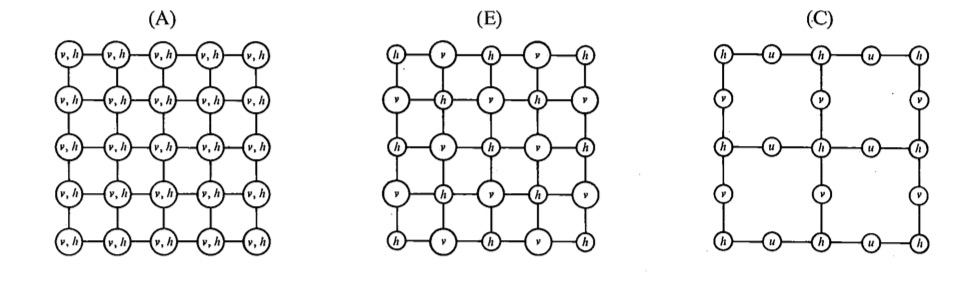
\includegraphics[keepaspectratio]{./pictest/pic421.jpg}}
\caption{}
\end{figure}

We shall denote the shortest distance between the grid points by
\(d^{*}\). With the same value of \(d^{*}\) the lattice (E) will have
twice, and the lattice (C) four times less variables per unit area than
the lattice (A), as in \texttt{figg:421}. The lattice (E) can be
obtained by a superposition of two (C) lattices, and the lattice (A) by
a superposition of two (E) lattices, or of four (C) lattices.

The admissible regions of wave numbers in the wave number plane can be
found by considering the shortest resolvable wave lengths. Note that
with lattice (E) the lines joining the nearest points with the same
variable make an angle of \(\frac{\pi}{4 }\) with the grid lines while
with the other two lattices these lines are along the grid lines.
\texttt{figg:422} shows the admissible wave numbers. A halving of the
number of variables is associated with a halving of the area of the
admissible region of the wave number plane.

The same standard finite difference approximations can be used for the
space derivatives in \texttt{b2.1} for all three lattices. We write
these approximations using the difference operators \(\delta_{x} \) and
\(\delta_{y}\), defined by, for example,

\[\delta_x h = \frac{1}{2d^*}\left[ h(x+d^*,y) - h(x-d^*,y)  \right]\]

Thus, \texttt{b2.1} can be approximated by

{\[\frac{\partial u}{\partial t} &= - g\delta_{x}h\]\[\frac{\partial v}{\partial t} &= - g\delta_{y}h\]\[\frac{\partial h}{\partial t} &= - H\left( \delta_{x}u + \delta_{y}v \right)\]}

Substituting wave solutions analogous as in \texttt{b2.2}, we obtain

{\[v^2 = gH\frac{\sin^{2}{kd^*} + \sin^2{l d^*}{d^{*2}}\]}

we define

\[X \equiv kd^{*} \qquad Y \equiv ld^{*}\]

% \begin{figure}
% \centering
% 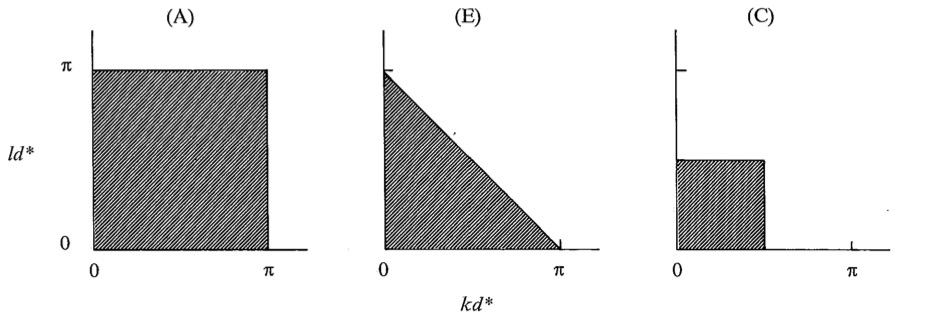
\includegraphics[width = .5 \textwidth]{./figs/GD/pic422.jpg}
% \caption{}
% \label{fig:}
% \end{figure}

\begin{description}
\item[the ratio of the phase speed given by \texttt{b2.5}, \(c^*\) to
the true phase speed]
\(\sqrt{gH}\) , can be written as
\end{description}

{\[\frac{c^*}{ \sqrt{gH}} = \sqrt{\frac{\sin^{2}X + \sin^{2}Y}{X^{2} + Y^{2}}}\]}

This formula reduces to the previous formula, \texttt{b1.8} or
\texttt{b1.9}, when applied to the one-dimensional case.

The values of the relative phase speed \texttt{b2.6} on the wave number
region admitted by lattice (E) are shown in \texttt{figg:423}. By
symmetry about the line \(l = k\) only half of the region needs to be
shown. \texttt{figg:422} shows that lattice (C) admits only the left
half of the triangular region

% \begin{figure}
% \centering
% 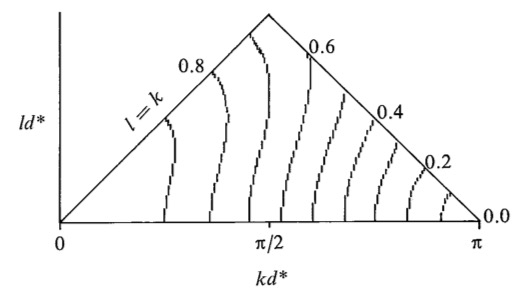
\includegraphics[keepaspectratio]{./figs/GD/pic423.jpg}
% \caption{}
% \label{fig:}
% \end{figure}

shown in the diagram. Clearly lattice (C) gives a more accurate phase
speed for gravity waves than the other lattices considered here.
Unfortunately, because it does not carry the two velocity components at
the same points, there is some difficulty with the Coriolis force term.
Of the other lattices, the staggered lattice (E) is much superior to the
non-staggered lattice (A). A result with the same truncation error can
be achieved in about half of the computation time, (exactly half if the
equations are linear), and a sizable fraction of wave numbers that are
associated with large phase speed errors and compu­tational dispersion
are eliminated. The additional time needed for a calculation on an (A)
lattice is spent on waves that can hardly be expected to improve the
inte­gration.

As we can see from the phase speed diagram, lattice (E) is not free of
computational problems.

As with the non-staggered one-dimensional grid discussed in the
preceding section, the solutions of \texttt{b2.4} on each of the two
type (C) subgrids forming the (E) lattice are inde­pendent and can
diverge from each other. This can be a source of serious problems. For
example, if the values of the dependent variables on one of these (C)
lattices are constant, they will be a stationary solution on that
lattice, no matter what the values of the variables on the other (C)
lattice are. Two stationary solutions, with different constant values on
each of these complementary lattices, will give a stationary wave
represented by the right-hand corner of the triangular region in
\texttt{figg:423}, with a zero phase speed. This wave is usually
referred to as the \emph{two-grid-interval wave}. In the same way, the
(A) lattice admits four independent stationary solutions, with different
constant values on each of its four type (C) subgrids.

The two-grid-interval wave can easily be generated when boundary
conditions are artificially described, and, with more complete
equations, in cases when gravity waves are generated inside the
computational region. These can be caused by heating, for example
through the release of latent heat, and by the influence of mountains.
When gravity waves are excited involving variables of one of the (C)
subgrids only, for example by forcing at individual grid points or lines
of points, the gravity wave will propagate through the variables of this
subgrid only. The variables of the other (C) subgrid will be influenced
only through the Coriolis and advection terms on a much larger
time-scale. Thus physical effects which may excite relatively long waves
in the atmosphere may excite spurious waves with wave lengths of
approximately two grid intervals in a computation. When these reach an
excessive amplitude, some remedial measures have to be taken. These will
be discussed in a later section.

\subsection{\texorpdfstring{\textbf{Gravity-inertia waves and space
distribution of
variables}}{Gravity-inertia waves and space distribution of variables}}\label{Section4.3}

In this section we discuss the effect of centered space differencing on
\emph{gravity-inertia waves}. Thus, we consider the system of linearized
equations

{\[\frac{\partial u}{\partial t} &= - g\frac{\partial h}{\partial x} +f v\]\[\frac{\partial v}{\partial t} &= - g\frac{\partial h}{\partial y} - f u\]\[\frac{\partial h}{\partial t} &= - H\nabla\cdot\textbf{v}\]}

These equations differ from those of section \texttt{Section4.2} in the
appearance of the two Coriolis terms. The Coriolis terms contain no
derivatives. However, they are difficult to calculate on the (C)
lattice, which was ideal for pure gravity waves.

Thus, we reconsider the problem of the distribution of the variables.

It is not obvious how we should analyse various arran­gements of
variables. Our primary concern here is to consider \texttt{b3.1} as part
of the complete system of primitive equations. We are interested in
large-scale motions, otherwise we would not be including the Coriolis
terms.

On the large scale, the primitive equations admit two district types of
motion : low-frequency, quasi-geostrophic and quasi-nondivergent flow
and high-frequency gravity-inertia waves. Gravity-inertia waves are
continually excited in the atmosphere. However, as they are dispersive,
a local accumulation of wave energy disperses with time. This process is
known as geostrophic adjustment; the remaining motion is in approximate
geostrophic balance and changes only slowly in time. In this chapter we
are concerned with the correct simulation of this process, which is
essentially governed by the gravity-inertia wave equations
\texttt{b3.1}.

We are interested both in waves caused by physical effects, and in those
caused by inadequacies of the initial data and of the numerical
procedures.

However, the details of the adjustment process do not matter as much as
the correctness of the resulting quasi-geostrophic flow.

We shall therefore investigate the effect of the space distribution of
dependent variables on the dispersive properties of the gravity-inertia
waves. This will be done using the simplest centered approximations for
the space derivatives, leaving the time derivatives in their
differen­tial form.

The discussion is based on that by Winninghoff and Arakawa, as presented
by Arakawa (Arakawa, 1972; Arakawa et al. 1974).

We consider five ways of distributing the dependent variables in space,
shown in \texttt{figg:431}. We denote by \emph{d} the shortest distance
between neighbouring points carrying the same dependent variable. In the
figure \emph{d} is the same for each of the five lattices ; thus, all
the lattices have \emph{the same number of dependent variables per unit
area}. The computation time needed for an integration on each of the
lattices will be about the same; the properties of the solution
obtained, though, will differ because of the effect of the space
arrangement of variables.

Using the subscripts shown in the figure, we define the centered space
differencing operator by

\[(\delta_x\alpha) = \frac{1}{d'} \left( \alpha_{i+\frac{1}{2},j} - \alpha_{i-\frac{1}{2},j} \right)\]

this rotation is applicable to all the lattices. Here \(d^{'}\) is the
distance between the points between which the finite difference is
taken. Thus, for lattices (A) through (D) \(d^{'}\) is equal to the grid
size \(d\), and for the lattice (E) it is equal to \(\sqrt{2d}\).

% \begin{figure}
% \centering
% \pandocbounded{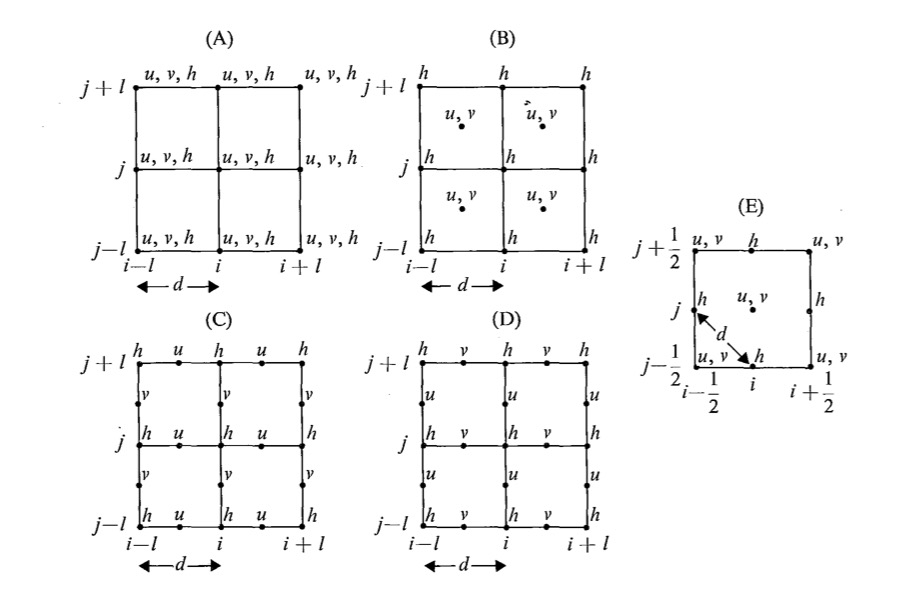
\includegraphics[keepaspectratio]{./pictest/pic431.jpg}}
% \caption{}
% \end{figure}

We also define an average taken over the same two points by

\[\left( {\overline{\alpha}}^{x} \right)_{i,j} \equiv \frac{1}{2}\left( \alpha_{i + \frac{1}{2},j} - \alpha_{i - \frac{1}{2},j} \right)\]

\(\left( \delta_{y}\alpha \right)_{i,j}\) and
\(\left( {\overline{\alpha}}^{y} \right)_{i,j}\) are defined in the same
way, but with respect to the \emph{y} axis. Finally,

\[\left( {\overline{\alpha}}^{xy} \right)_{i,j}  \equiv  \left( {\overline{\overline{\alpha}}^{x}}^y \right)_{i,j}\]

For each of the five lattices we use the simplest centered
approximations for the space derivatives and Coriolis terms
\texttt{b3.1}. We obtain the difference systems

{\[\frac{\partial u}{\partial t} &= - g\overline{\delta_x h}^{x} + fv\]\[\frac{\partial v}{\partial t} &= - g\overline{\delta_y h}^{y} - fu\]\[\frac{\partial h}{\partial t} &= -H\left( \overline{\delta_x u}^{x} + \overline{\delta_y v}^{y} \right)\]}

{\[\frac{\partial u}{\partial t} &= - g\overline{\delta_x h}^{y} + fv\]\[\frac{\partial v}{\partial t} &= - g\overline{\delta_y h}^{x} - fu\]\[\frac{\partial h}{\partial t} &= -H\left( - \overline{\delta_x u}^{y} +  \overline{\delta_y v}^x \right)\]}

{\[\frac{\partial u}{\partial t} &= - g\delta_x h + f\overline{v}^{xy}\]\[\frac{\partial v}{\partial t} &= - g\delta_y h - f\overline{u}^{xy}\]\[\frac{\partial h}{\partial t} &= -H\left( \delta_x u +  \delta_y v \right)\]}

{\[\frac{\partial u}{\partial t} &= - g\overline{\delta_x h}^{xy} + f\overline{v}^{xy}\]\[\frac{\partial v}{\partial t} &= - g\overline{\delta_y h}^{xy} - f\overline{u}^{xy}\]\[\frac{\partial h}{\partial t} &= -H\left( \overline{\delta_x u}^{xy} 
+  \overline{\delta_y v}^{xy} \right)\]}

{\[\frac{\partial u}{\partial t} &= - g\delta_x h + fv\]\[\frac{\partial v}{\partial t} &= - g\delta_y h - fu\]\[\frac{\partial h}{\partial t} &= -H\left( \delta_x u +  \delta_y v \right)\]}

We shall first analyze a one-dimensional case, that in which the
variables, \(u,v \) and h do not vary with \(y\)

Thus, we have

\begin{quote}
\(u,v,h = u,v,h\left( x,t \right)\)
\end{quote}

The system \texttt{b3.1} then reduces to

{\[\frac{\partial u}{\partial t} &= -g\frac{\partial h}{\partial x} + fv\]\[\frac{\partial v}{\partial t} &= - fu\]\[\frac{\partial h}{\partial t} &= -H\frac{\partial u}{\partial x}\]}

Substituting the wave solutions \texttt{b1.2}, we obtain the frequency
equation which can be written as

{\[\left( \frac{\nu}{f} \right)^{2} = 1 + \frac{gH}{f^{2}}k^{2}\]}

Thus, as the \emph{radius of deformation}

\[\lambda = \sqrt{\frac{gH}{f}}\]

is never equal to zero, the frequency of the gravity-inertia waves is a
monotonically increasing function of \(k\). Therefore, the group
velocity \(\frac{\partial\nu}{\partial k}\) is never equal to zero. This
is very important for the geostrophic adjust­ment process, as it
precludes a local accumulation of wave energy.

We now look at the effect of the finite differencing in space in this
case. As the variables are assumed not to depend on \(y\), the systems
\texttt{b3.2A} reduce to

{\[\frac{\partial u}{\partial t} &= - g\overline{\delta_x h}^{x} + fv\]\[\frac{\partial v}{\partial t} &=  - fu\]\[\frac{\partial h}{\partial t} &= -H \overline{\delta_x u}^{x}\]}

{\[\frac{\partial u}{\partial t} &= - g\delta_x h + fv\]\[\frac{\partial v}{\partial t} &=  - fu\]\[\frac{\partial h}{\partial t} &= -H \delta_x u\]}

{\[\frac{\partial u}{\partial t} &= - g\delta_x h + f\overline{v}^{x}\]\[\frac{\partial v}{\partial t} &=  - f\overline{u}^{x}\]\[\frac{\partial h}{\partial t} &= -H \delta_x u\]}

{\[\frac{\partial u}{\partial t} &= - g\overline{\delta_x h}^{x} + f\overline{v}^{x}\]\[\frac{\partial v}{\partial t} &=  - f\overline{u}^{x}\]\[\frac{\partial h}{\partial t} &= -H \overline{\delta_x u}^{x}\]}

{\[\frac{\partial u}{\partial t} &= - g\delta_x h + fv\]\[\frac{\partial v}{\partial t} &=  - fu\]\[\frac{\partial h}{\partial t} &= -H \delta_x u\]}

Substitution of wave solutions into these systems gives the frequency
equations

{\[\left(\frac{\nu}{d}\right)^2 = 1 + \left(\frac{\lambda}{d}\right)^2 \sin^2{kd}\]}

{\[\left(\frac{\nu}{d}\right)^2 = 1 + 4\left(\frac{\lambda}{d}\right)^2 \sin^2{\frac{kd}{2}}\]}

{\[\left(\frac{\nu}{d}\right)^2 = \cos^2{\frac{kd}{2}} + 4\left(\frac{\lambda}{d}\right)^2 \sin^2{\frac{kd}{2}}\]}

{\[\left(\frac{\nu}{d}\right)^2 = \cos^2{\frac{kd}{2}} + \left(\frac{\lambda}{d}\right)^2 \sin^2{\frac{kd}{2}}\]}

{\[\left(\frac{\nu}{d}\right)^2 = 1 + 2\left(\frac{\lambda}{d}\right)^2 \sin^2{\frac{kd}{\sqrt{2}}}\]}

The non-dimensional frequency \(\frac{\nu}{f}\) is now seen to depend on
two parameters, \(kd\) and \(\frac{\lambda}{d}\)

We shall analyze the dispersion properties revealed by these expressions
for each of the five lattices. The wavelength of the shortest resolvable
wave along the \(x\) axis is \(2d\) for lattices (A) through (D), and
\(\sqrt{2d}\) for the lattice (E). Thus, we have to consider the range
\(0 < kd \leq \pi\) for lattices (A) through (D), and the range
\(0 < kd \leq \sqrt{2\pi}\) for the lattice (E).

Lattice (A): The frequency reaches a maximum a \( kd = \frac{\pi}{2}\)
Thus, the group velocity is zero for \(k\) equal to
\(\frac{\pi}{\left( 2d \right)}\). If gravity-inertia waves of
approximately that wave number are excited near a point inside the
computa­tional region, for example by nonlinear effects or forcing
through heating or ground topography, the wave energy stays near that
point. Beyond this maximum value, for \(\frac{\pi}{2 < kd < \pi}\), the
frequency decreases as the wave number increases. Thus, for these waves
the group velocity has the wrong sign. Finally, the two-grid-interval
wave with \(kd = \pi\) behaves like a pure inertia oscillation, and its
group velocity is again zero.

Lattice (B): The frequency increases monotonically throughout the range
\(0 < kd < \pi\) . However, it reaches a maximum at the end of the
range, so that the group velocity is zero for the two-grid-interval wave
with \(kd = \pi.\)

Lattice (C): The frequency increases monotonically with \(\text{kd}\) if
\(\frac{\lambda}{d} > \frac{1}{2} \) and decreases monotonically with
\(\text{kd}\) if \(\frac{\lambda}{d} < \frac{1}{2}\). It again reaches
an extreme value at \(kd = \pi\), associated with a zero group velocity.
For \(\frac{\lambda}{d} = \frac{1}{2}\) the group velocity is equal to
zero for all \(k\) .

Lattice (D): The frequency reaches a maximum at
\(\left( \frac{\lambda}{d} \right)^{2}\cos{kd} = \frac{1}{4}\). The
two-grid-interval wave at \(kd = \pi\) is stationary.

Lattice (E): The frequency reaches a maximum at
\(kd = \frac{\pi}{\sqrt{2}}\). The shortest resolvable wave with
\(kd = \sqrt{2\pi}\) behaves like a pure inertia oscillation, and its
group velocity is again zero.

A summary of these results is shown in \texttt{figg:432}. It shows the
functions \(\frac{|v|}{f}\), in the case \(\frac{y}{d} = 2\).

% \begin{figure}
% \centering
% \pandocbounded{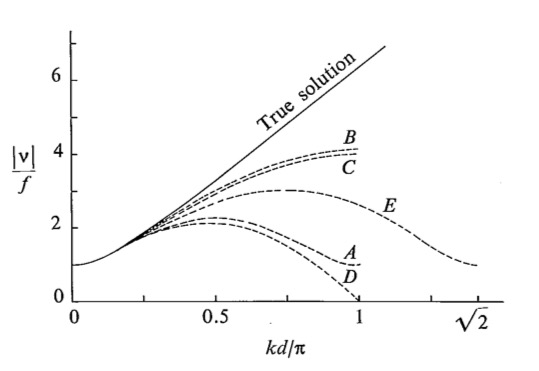
\includegraphics[keepaspectratio]{./pictest/pic432.jpg}}
% \caption{}
% \end{figure}

The figure vividly illustrates the inadequacy of the lattices (D) and
(A). The phase speed and dispersion properties of the remaining three
lattices are much better: however, zero group velocities occur with
every lattice. Thus, with any lattice there will be difficulties in the
geostrophic adjustment process.

The difference between the results for lattices (B) and (E) is
interesting because these two lattices can be obtained from one another
by a rotation through an angle of \(\frac{\pi}{4}\) If we consider the
one-dimensional case in which the dependent variables are constant along
the lines \(y = x + c\), we obtain results for these two lattices that
are exactly opposite to those in\texttt{figg:432}. In general, we define
the coordinate system \emph{x\textquotesingle, y\textquotesingle{}} by
rotating the \emph{x,y} in the positive direction through an angle of
\(\frac{\pi}{4}\), and then, using the relations

\[u^{'} &= \frac{\sqrt{2}}{2}\left( u + v \right)\]\[v^{'} &= \frac{\sqrt{2}}{2}\left( - u + v \right)\]

change from variables \(u,v,h\) to new dependent variables
\(u^{'},v^{'},h\) . We find that this transforms the system
\texttt{b3.2B} into \texttt{b3.2E}, and, conversely, \texttt{b3.2E} into
\texttt{b3.2B}. Thus, the \emph{dispersion properties of the lattices
(B) and (E) can be considered equivalent}. A gravity-inertia wave in one
of these lattices has phase speed and dispersion properties identical to
those of the same wave with its front rotated through an angle of
\(\frac{\pi}{4}\) in the other lattice.

Obviously, we should also consider the two-dimensional case. The values
of \(\frac{|v|}{f}\) that are obtained in the two-dimensional case for
the true solution and those using lattices (B) and (C) are shown in
\texttt{figg:433} with \(\frac{\lambda}{d'} = 2\). The diagram for
lattice (E) can be obtained by a counter­clockwise rotation of the (B)
lattice diagram.

% \begin{figure}
% \centering
% \pandocbounded{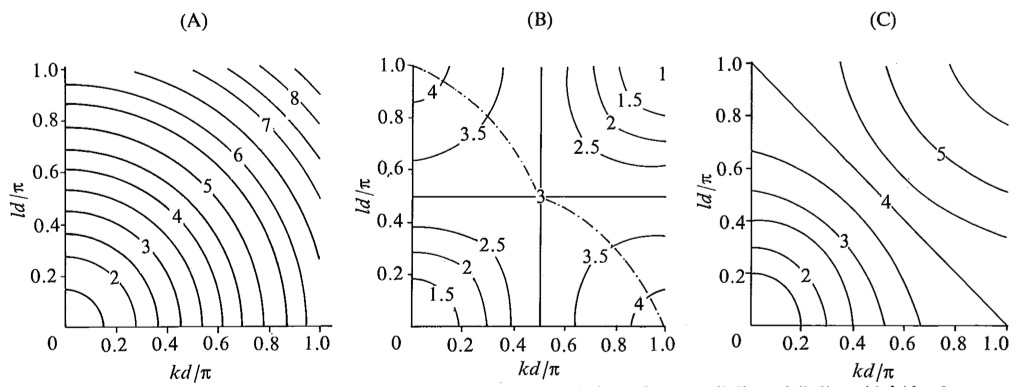
\includegraphics[keepaspectratio]{./pictest/pic433.jpg}}
% \caption{}
% \end{figure}

The diagram for lattice (C) in the two-dimensional case is seen to be a
much better approximation to the exact solution than the (B) or (E)
lattice diagram. In the (B) lattice diagram the dot-dashed line shows
the maximum \(\frac{|v|}{f}\) for a given ratio \(\frac{l}{k}\); note
that there is no such line in the (C) lattice diagram and the exact
solution. Such a maximum occurs at only two corner points of the (C)
lattice diagram. Thus, with the (C) lattice, no waves have a group
velocity with the wrong sign. The situation, though, does depend on the
parameter \(\frac{\lambda}{d}\). With a stra­tified atmosphere the
radius of deformation \(\lambda\). depends on the stability ; if the
stability is so weak as to make \(\frac{\lambda}{d}\) of the order of 1
or less, the (C) lattice loses the advantages shown in
\texttt{figg:433}. However, for typical grid sizes used in atmospheric
models this is not the case and therefore Arakawa (Arakawa and Lamb,
1976) concludes that the lattice (C) is the best lattice to simulate the
geostrophic adjustment process. Accordingly, it is at present being used
in the general circulation model at the University of California at Los
Angeles, and also in the British operational model.

The (B) or (E) lattices have a problem with false low frequencies of the
shortest waves. The two-grid-interval wave, that was stationary as a
pure gravity wave, now behaves like a pure inertia oscillation. The
difficulty arises from decoupling of the gravity wave solutions on the
two complementary (C) type subgrids. Methods of dealing with this will
be discussed later.

\subsection{\texorpdfstring{\textbf{Time differencing; the leapfrog
scheme and the Eliassen
grid}}{Time differencing; the leapfrog scheme and the Eliassen grid}}\label{Section4.4}

Properties of time differencing schemes applied to the gravity wave
equations can be deduced from the analysis of Chapter \texttt{Chapter2},
as was done for the advection equation.

We shall demonstrate this for the one-dimensional equations

{\[\frac{\partial u}{\partial t} + c\frac{\partial u}{\partial x} +
 g\frac{\partial h}{\partial x} &= 0\]\[\frac{\partial h}{\partial t} + c\frac{\partial h}{\partial x} +
 H\frac{\partial u}{\partial x} &= 0\]}

We first multiply the second of these equations by an arbitrary
parameter \(\lambda\), and add the result to the first equation. We
obtain

{\[\frac{\partial}{\partial t}( u + \lambda h ) +
( c + \lambda H )\frac{\partial u}{\partial x} +
( g + \lambda c )\frac{\partial h}{\partial x} = 0\]}

We wish to choose \(\lambda\) so that

{\[\frac{g + \lambda c}{c + \lambda H} = \lambda\]}

\begin{description}
\item[to obtain an equation with only one dependent variable,]
\(u + \lambda h\) . The two solutions of \texttt{b4.3} are
\end{description}

{\[\lambda = \pm \sqrt{\frac{g}{H}}\]}

Substituting these into \texttt{b4.2} we obtain

{\[\left[ \frac{\partial}{\partial t} + ( c + \sqrt{gH}\frac{\delta}{\text{δx}} ) \right] \left( u + \sqrt{\frac{g}{H}}h \right) &= 0\]\[\left[ \frac{\partial}{\partial t} + ( c - \sqrt{gH}\frac{\delta}{\text{δx}} ) \right] \left( u - \sqrt{\frac{g}{H}}h \right) &= 0\]}

This is the \emph{normal form} of the system \texttt{b4.1}. It shows
that \texttt{b4.1} is equivalent to a system of two advection
equations*. The quantity \(u + \sqrt{\frac{g}{H}}h\) is seen to be
advected at a velocity \(c + \sqrt{gH}\) in the direction of the
\(\text{x }\) axis, while, at the same time, the quantity
\(u - \sqrt{\frac{g}{H}}h\) is advected in the same direction at a
velocity \(c - \sqrt{gH}\).

Suppose now we choose a grid that carries both u and h at every grid
point. The systems obtained by using centered space differencing in
\texttt{b4.1} and \texttt{b4.5} are then equivalent. We can therefore
use the same procedure as in Section 1 of the Chapter \texttt{Chapter3}
to analyse time differencing schemes. We obtain the same results as
before, except that in place of the advection velocity \(c\) we now have
\(c + \sqrt{gH}\). Thus, if the \emph{leapfrog scheme} is used for the
time differencing, and \(c\) is considered positive, we obtain the
Courant-Friedrichs-Lewy stability criterion for this case as

{\[( c + \sqrt{gH})\frac{\Delta t}{\Delta x} \leq 1\]}

The advection velocity in the atmosphere is normally about an order of
magnitude less than the phase speed of external gravity waves.
Accordingly, in the foregoing criterion \(c\) is often neglected
compared with \(\sqrt{gH}\), giving the stability requirement

{\[\sqrt{gH}\frac{\Delta t}{\Delta x} < 1\]}

When using the \emph{three-dimensional} primitive equations, external
gravity waves are normally eliminated by per­mitting no vertical
velocity at the upper boundary. The highest phase speed admitted by the
system is then that of the Lamb waves, which for an isothermal
atmosphere is

\[\sqrt{\left( \frac{f}{k} \right)^{2} + \gamma RT}\]

where \(\gamma \equiv \frac{c_{p}}{c_{v}}\). If we neglect the first
term and recall that the scale height of an isothermal atmosphere is

\[H^{*} = \frac{RT}{g}\]

we see that the phase speed of the Lamb waves is of the same order of
magnitude as that of the external gravity waves. Thus, in view of the
relation between stability and the phase speed, we see that
\texttt{b4.7} should also repre­sent an approximately correct stability
requirement in the three-dimensional case. With the highest phase speeds
of the order of 300 m \(\text{sec}^{-1}\), and a grid size of about 100
km, this requirement does not permit time steps longer than about 5
minutes. This time will be smal­ler by a factor of \(\sqrt{2}\) with two
horizontal coordinates. The CFL stability condition thus means that a
large amount of computer time is required for integration of the
primitive equations, especially when the grid size is small to reduce
errors in space differencing. For this reason some investigators prefer
using implicit time dif­ferencing schemes, so that the choice of time
step can be based solely on accuracy and not on stability.

We can also study the stability and other properties of time
differencing methods applied to the gravity wave equations by direct
substitution of wave solutions. For example, consider the leapfrog
scheme with centered space differencing applied to the
\emph{two-dimensional} system

{\[\frac{\partial u}{\partial t} + g\frac{\partial h}{\partial x} = 0\]\[\frac{\partial v}{\partial t} + g\frac{\partial h}{\partial y} = 0\]\[\frac{\partial h}{\partial t} + H\nabla\cdot v = 0\]}

Using one of the lattices of \texttt{figg:421} as well as the notation
of Section \texttt{Section4.2}, we obtain

{\[u^{n+1} = u^{n-1} -2 g \Delta t \delta_x h^n\]\[v^{n+1} = v^{n-1} -2 g \Delta t \delta_y h^n\]\[h^{n+1} = h^{n-1} -2 H \Delta t ( \delta_x u + \delta_y v)^n\]}

Substituting the wave solutions

{\[u^n = Re \left[ \lambda^n \widehat{u} e^{i(kx+ly)} \right]\]\[v^n = Re \left[ \lambda^n \widehat{v} e^{i(kx+ly)} \right]\]\[h^n = Re \left[ \lambda^n \widehat{h} e^{i(kx+ly)} \right]\]}

we obtain the homogeneous system

{\[\left( \lambda^{2} - 1 \right)\widehat{u} + i\lambda 2\sqrt{2}g\mu \sin{X}\widehat{h} = 0\]\[\left( \lambda^{2} - 1 \right)\widehat{v} + i\lambda 2\sqrt{2}g\mu \sin{Y}\widehat{h} = 0\]\[i\lambda 2\sqrt{2}K\mu \left( \sin{X}\widehat{u} + \sin{Y}\widehat{v} \right) + \left( \lambda^{2} - 1 \right)\widehat{h} = 0\]}

Here \emph{X} and \emph{Y} are defined as in Section \texttt{Section4.2}
, while

\[\mu \equiv \frac{\Delta t}{\left( \sqrt{2}d^{*} \right)}\]

that is, \(\mu \equiv \frac{\Delta t}{d}\) when the lattice (E) is
chosen.

The properties of the numerical solution can now be studied by analyzing
\texttt{b4.11}. The requirement that its determinant be equal to zero
gives six solutions for \(\lambda\). Two of these are

{\[\lambda = 1\]}

and

{\[\lambda = - 1\]}

The remaining four are given by

{\[\lambda^{2} = 1 - 4A \pm 2\sqrt{2A( 2A - 1 )}\]}

Where

\[A \equiv gH\mu^{2}\left( \sin^{2}X + \sin^{2}Y \right)\]

We can now analyze the solutions \texttt{b4.10} associated with the
values found for \(\lambda\). The first of these values, \texttt{b4.12},
gives a neutral and stationary solution. If either \(\sin{X}\) or
\(\sin{Y}\) is non-zero in this neutral and stationary case then,
according to \texttt{b4.11}, we have \(\widehat{h} = 0\), and the
solution represents a physically acceptable translatory motion. If,
however, sin \(X\) and \(\sin{Y}\) are both equal to zero, the
amplitudes of all three dependent variables can take arbitrary values.
In addition to the physically acceptable solution where all the
dependent variables are constant \(\left( k = l = 0 \right)\) there is a
solution with one or both of the wave numbers \(k\) and \(l\) equal to
\(\frac{\pi}{d^{*}}\). This is the two-grid-interval wave, discussed
already in Section \texttt{Section4.2}. It again appears as a false
computational solution; since it is stationary, it is not affected by
the introduction of time differencing.

The second value, \(\lambda = - 1\), represents a false compu­tational
mode in time, with a period of \(2\Delta t\). This com­putational mode
results from using a three time level scheme.

To prove stability of the scheme the behaviour of the remaining
solutions given by \texttt{b4.14} has to be investigated. They will all
also be neutral for \(2A < 1\). To obtain the condition in the form
\(B\Delta t \leq 1\) we write

\[\sqrt{2A \leq 1}\]

Since this has to be satisfied for all the admissible waves, we find
that the CFL criterion in the two-dimensional case is now

{\[2\sqrt{gH}\mu \leq 1\]}

or

{\[\sqrt{2gH}\frac{\Delta t}{\Delta x} \leq 1\]}

This is in agreement with the previous results. The non dimensional
constant on the left side is sometimes called the \emph{Courant number}.

With solutions like \texttt{b4.10}, the frequency \(\text{v }\) is given
by

\[\lambda = \left| \lambda \right|e^{- i\nu\Delta t}.\]

Thus, the expressions obtained for \(\lambda\) can be used to calcu­late
the \emph{relative phase speed} \(\frac{c^{*}}{\sqrt{gH}}\) using the
relation

{\[\frac{c^{*}}{\sqrt{gH}} = \frac{1}{\Delta t\sqrt{gH\left( k^{2} + l^{2} \right)}}\arctan\frac{- \lambda_{im}}{\lambda_{re}}\]}

If we are given \(\lambda^{2}\) rather than \(\lambda\), as here, we can
express the relative phase speed as a function of \((\lambda^{2})_{im}\)
and \((\lambda^{2})_{re}\). Thus, using \texttt{b4.14}, we find for
\(2A \leq 1:\)

{\[\frac{c^*}{\sqrt{gH}} = \frac{1}{2\mu\sqrt{2gH\left( X^{2} + Y^{2} \right)}} \times
 \arctan{ \left( \pm \frac{2\sqrt{2A\left( 1 - 2A \right)}}{1 - 4A} \right)   }\]}

\begin{description}
\item[This expression, of course, approaches \texttt{b2.6} as]
\(\Delta t\) approaches zero.
\end{description}

For a more explicit illustration of the effect of time differencing, we
can perform a series expansion of \texttt{b4.18}. One obtains, for
\(\sqrt{2A} < \frac{1}{\sqrt{2}},\)

\[\frac{c^*}{\sqrt{gH}} = 
\sqrt{\frac{\sin^2{X} + \sin^2{Y}}{X^2 + Y^2}} \left( 1 + \frac{1}{3}A + \frac{3}{10}A^2 + \ldots \right)\]

The factor multiplying the series in parenthesis describes the
decelerating effect of space differencing, as given by \texttt{b2.6}.
The acceleration resulting from the leapfrog time differencing is
beneficial, as it reduces the phase error due to space differencing.

The values of the relative phase speed \texttt{b4.18} are shown in
\texttt{figg:441}, for the physical mode with \( 2\sqrt{gH\mu} = 0.5\).
The wave number region shown here is the same as in \texttt{figg:423},
where the effect of space differencing alone was considered. Comparison
of these figures shows little difference between the two families of
isolines. The relative acceleration due to the time differencing has a
maximum at the upper corner of the diagram, but the relative phase speed
here is still poor.

% \begin{figure}
% \centering
% \pandocbounded{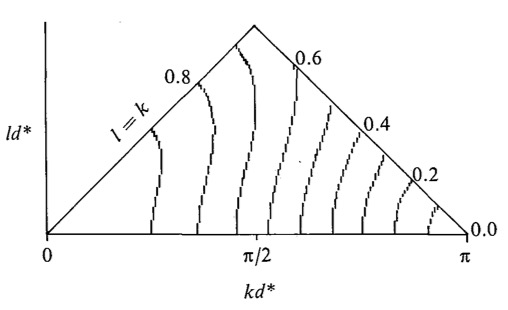
\includegraphics[keepaspectratio]{./pictest/pic441.jpg}}
% \caption{}
% \end{figure}

Finally, we point out that time differencing suggests new ways of
distributing the variables, as the grid can now also be time-staggered.
A good example is given by the linearized system

{\[\frac{\partial u}{\partial t} + g\frac{\partial h}{\partial x} - fv &= 0\]\[\frac{\partial v}{\partial t} + g\frac{\partial h}{\partial y} + fu &= 0\]\[\frac{\partial h}{\partial t} + H\left( \frac{\partial u}{\partial x} + \frac{\partial v}{\partial y}  \right) &= 0\]}

approximated using lattice (E), the leapfrog scheme and centered space
differencing. If all the variables were calculated at every time level,
there would be two inde­pendent solutions. The solution involving the
variables of the space-time grid shown in \texttt{figg:442} would be
indepen­dent of that involving the variables that are left out in this
figure. The second grid can be obtained by shifting the grid a distance
\(\sqrt{2d^{*}} \) along the line \( y = x.\) Thus, as with the space
grids discussed in Section \texttt{Section4.2}, the space-time grid
formed by using the (E) lattice at every time level can be considered as
a superposition of two element­ary subgrids of the type shown in
\texttt{figg:442}. Solving the system \texttt{b4.19} on only one of
these saves half the computa­tion time, with no change in the truncation
error. In addition the computational mode in time, given by
\texttt{b4.13}, is eliminated, as the variables at alternate time levels
are missing. Thus, with a more complete system of equations, the gradual
separation of solutions at alternate time levels is not possible. The
advantages of the space-time grid shown in the figure were pointed out
by Eliassen (1956) at an early stage in the study of the primitive
equations, and it is called the \emph{Eliassen grid.}

However, as pointed out by Platzman (1958 ; 1963) the grid in
\texttt{figg:442} can again be considered as formed by a superposition
of two subgrids, where in each of these subgrids only the height is kept
at one time level and the velocity components at the next. Platzman
calls this sub­grid the \emph{Richardson grid}. A single Richardson grid
is considered as a time-staggered version of the (C) lattice and
suffices for the solution of the pure gravity wave system \texttt{b4.9}
; thus, on an Eliassen grid the system \texttt{b4.9} has two independent
solutions. Using the difference system considered above to approximate
the differential system \texttt{b4.19}, these solutions are coupled only
through the two Coriolis terms.

% \begin{figure}
% \centering
% \pandocbounded{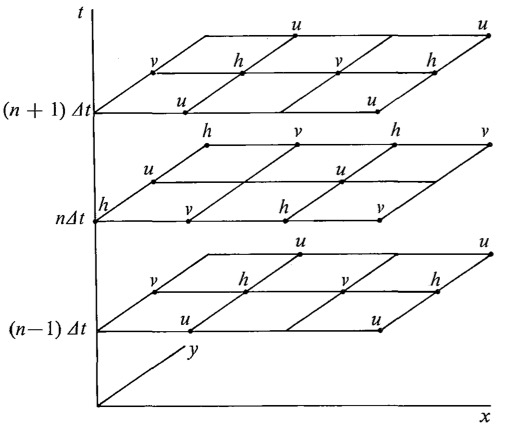
\includegraphics[keepaspectratio]{./pictest/pic442.jpg}}
% \caption{}
% \end{figure}

\subsection{\texorpdfstring{\textbf{Economical explicit
schemes}}{Economical explicit schemes}}\label{economical-explicit-schemes}

The fact that we are now solving two equations, the equation of motion
and the continuity equation, sug­gests new ways of constructing time
differencing sche­mes. Some of these have recently attracted the
attention of atmospheric modellers.

As seen in the section \texttt{Section4.4}, an inconvenient feature of
gravity waves is the high computer time required for a solution using
explicit schemes for the time differencing. The time step imposed by the
CFL stability criterion is generally considered to be much less than
that required for an accurate integration of the slower
quasi-geostro-phic motions. With these steps, the errors due to space
differencing are much greater than those due to time differencing.
Robert (1974), for example, estimates that the typical errors due to
space differencing in present atmospheric models amount to nearly 40 per
cent, and those due to time differencing only to about 1 per cent of the
total error. Thus, any economy that can be made in time differencing is
welcome, as the time that is saved can usefully be used to increase the
accuracy of the space differencing.

Two explicit schemes that are more economical than the standard leapfrog
scheme will be given here. They both achieve economy by using a
different integration procedure for the height gradient terms of the
equation of motion and for the divergence term of the continuity
equation. For brevity, we call these terms the \emph{gravity wave terms}
of the governing equations.

We shall discuss the properties of one of these "econo­mical" schemes in
some detail. It is obtained by first integrating the gravity wave terms
of \emph{either} the equation of motion or of the continuity equation
forward, and then those of the other equation backward in time. Thus,
this scheme could be called the \emph{forward-backward} scheme. With
centered space differencing, \texttt{b4.8} is approximated by

{\[u^{n + 1} = u^{n} - g\Delta t\delta_{x}h^{n}\]\[v^{n + 1} = v^{n} - g\Delta t\delta_{y}h^{n}\]\[h^{n + 1} = h^{n} - H\Delta t\left( \delta_{x}u + \delta_{y}v \right)^{n + 1}\]}

or by an analogous system in which the order of integra­tion is
reversed.

Substituting the wave solutions \texttt{b4.10} we find three solutions
for x. One of these,

{\[\lambda = 1\]}

gives again a neutral and stationary solution. The remaining two are

{\[\lambda = 1 - A \pm \sqrt{A\left( A - 2 \right)}\]}

where the quantity \(A\) is defined as in the preceding section.
Solutions \texttt{b5.2} and \texttt{b5.3} are obtained for both versions
of the scheme, that is, no matter which of the two equations — the
equation of motion or the conti­nuity equation — is first integrated
forward.

Examination of the amplification factors given by \texttt{b5.3} shows
that the scheme is stable and neutral for \(  A \leq 2\) , that is, for

\[\sqrt{2A} \leq 2\]

To satisfy this for all the admissible waves, we must have

{\[2\sqrt{gH} \mu \leq 2\]}

Thus, the forward-backward scheme is stable and neutral with time steps
\emph{twice those allowed by the CFL criterion for the leapfrog scheme}
(Ames, 1969).

The amplification factors of the forward-backward and of the leapfrog
scheme are equal within their regions of stability. We now compare their
effect on the phase speed by comparing the expression \texttt{b5.3}, for
the forward­backward scheme, with \texttt{b4.14}, for the leapfrog
scheme. The right-hand side of \texttt{b5.3}, with \(A\) replaced by
\(4A\), is equal to the right-hand side of \texttt{b4.14}. Because of
the definition of \(A\), this means that \(\lambda\) for the
forward-back­ward scheme is identical to \(\lambda^{2}\) for the
leapfrog scheme when time steps are used for the forward-backward scheme
\emph{twice as long as} those for the leapfrog scheme ! Thus, the
forward-backward scheme gives the same result using only half the
computation time needed for the leapfrog scheme. In addition, as a two
level scheme, it has no computational mode in time.

To understand this advantage of the forward-back­ward over the leapfrog
scheme we compare the finite difference analogues that these two schemes
give for the wave equation, since the system of gravity wave equa­tions
is equivalent to a single wave equation. Consider the one-dimensional
version of this system:

{\[\frac{\partial u}{\partial t} + g\frac{\partial h}{\partial x} = 0\]\[\frac{\partial h}{\partial t} + H\frac{\partial u}{\partial x} = 0\]}

Eliminating one of the variables u, h we obtain a wave equation

{\[\frac{\partial^{2} h}{\partial t^{2}} - gH\frac{\partial^{2} h}{\partial x^{2}} = 0\]}

We can perform the same elimination for each of the finite difference
schemes.

The forward-backward and space-centered approxi­mation to \texttt{b5.5}
is

{\[\frac{u_j^{n + 1} - u_j^n}{\Delta t} + g\frac{h_{j + 1}^{n} - h_{j - 1}^{n}}{2\Delta x} = 0\]\[\frac{h_j^{n + 1} - h_j^n}{\Delta t} + H\frac{u_{j + 1}^{n + 1} - u_{j - 1}^{n + 1}}{2\Delta x} = 0\]}

We now substract from the second of these equations an analogous
equation for time level \(n - 1\) instead of \(n\), divide the resulting
equation by \(\Delta t\), and, finally, eliminate all u values from it
using the first of \texttt{b5.7}, written for space points \(j + 1\) and
\(j - 1\) instead of \(j\). We obtain

{\[\frac{h_{j}^{n + 1} - 2h_{j}^{n} + h_{j}^{n - 1}}{\left( \Delta t \right)} 
+ gH\frac{h_{j + 2}^{n} - 2u_j^{n} + h_{j - 2}^{n}}{\left( 2\Delta x \right)^{2}} = 0\]}

This is a finite difference analogue of the wave equation \texttt{b5.6}.
Note that although each of the two equations \texttt{b5.7} is only of
the first order of accuracy in time, the wave equation analogue
equivalent to \texttt{b5.7} is seen to be of the second order of
accuracy.

If we use a leapfrog and space-centered approximation to \texttt{b5.5},
and follow an elimination procedure like that used in deriving
\texttt{b5.8}, we obtain

{\[\frac{h_j^{n + 1} - 2h_ j^{n - 1} + h_j^{n - 3}}{\left( \Delta t \right)^{2}} 
- gH\frac{h_{j + 2}^{n - 1} - 2h_j^{n - 1} + h_{j - 2}^{n - 1}}{\left( 2\Delta x \right)^{2}} = 0\]}

This also is an analogue to the wave equation \texttt{b5.6} of
second-order accuracy. However, in \texttt{b5.8} the second time
derivative was approximated using values at three consecutive time
levels; in \texttt{b5.9} it is approximated by values at every second
time level only, that is, at time intervals \(2\Delta t\) . Thus, while
the time step required for linear stability with the leapfrog scheme was
half that with the forward-backward scheme, \texttt{b5.9} shows that we
can omit the variables at every second time step, and thus achieve the
same computation time as using the forward-backward scheme with double
the time step. This method was discussed in the previous section for the
two-dimensional case, it is the Eliassen grid. Thus, comparing
\texttt{b5.8} and \texttt{b5.9} shows that \emph{the economy
accomplished by the forward-backward scheme is equivalent to that
accomplished with leapfrog time differencing by the Eliassen grid}. Both
of these methods avoid calculating the false time computational mode,
and thus save half of the computation time with no effect on the
physical mode of the solution.

Comparing these two methods, the forward-backward scheme has some
advantages. With the forward-back­ward scheme all the variables are
defined at all grid points at every time step ; this facilitates the
programming work. In addition, the forward-backward scheme can be
modified to allow propagation of gravity waves between all points of the
grid preventing two-grid-interval noise. This modification will be
described in Section \texttt{Section4.8}. No analogous method, however,
has so far been proposed for the leapfrog scheme with the Eliassen grid.

A disadvantage of the forward-backward scheme is that it is not possible
to use the leapfrog scheme for the advection terms. However, the
second-order accurate Adams-Bashforth scheme can be used for these
terms. Its weak instability should cause no trouble because of the
relatively slow speed of the advection processes. For example, in
experiments of Mesinger and Janjic (1974), where a multi-level model was
used for simulation of the growth of a baroclinic wave, a forward scheme
was used for the advection terms, and no signs of insta­bility were
noticed for about a two week period. The forward-backward scheme has
been used for the storm surge problem by Fischer (1959) and Sielecki
(1968), and, in meteorology, by Gadd (1974) in experiments with the
British operational model.

Another way of constructing an economical explicit scheme was pointed
out by Shuman, Brown and Campana (1974), and it is now used in an
operational model at the National Meteorological Center. For the shallow
water equations with this scheme, the height values at time level
\(n + 1\) are first calculated using the leapfrog scheme, and then the
equation of motion is integrated using the height field averaged over
the time interval \(2\Delta t\) by the bi-trapezoidal rule :

\(\frac{1}{4}h^{n - 1} + \frac{1}{2}h^{n} + \frac{1}{4}h^{n + 1}\)

Substitution of wave solutions into the equations of this scheme gives
the value \texttt{b5.3} for \(\lambda\), in addition to the neutral
values. Thus, the stability criterion and the pro­perties of the
physical solution are the same as with the forward-backward scheme. Even
though this Shuman-Brown-Campana (SBC) scheme is a three level scheme,
time staggering of the grid is not possible because of the averaging of
the height values. Thus, the economy accomplished by the SBC scheme is
again equivalent to that accomplished with leapfrog time differencing by
the Eliassen grid. The SBC scheme has somewhat larger storage
requirements than the forward-backward scheme. However, it does permit
the use of the leapfrog scheme for the advection terms.

\subsection{\texorpdfstring{\textbf{Implicit and semi-implicit
schemes}}{Implicit and semi-implicit schemes}}\label{Section4.6}

The time step permitted by the economical explicit schemes, twice that
prescribed by the CFL criterion, is still considerably shorter than that
required for accurate integration of the quasi-geostrophic motions. Even
with these schemes the time differencing error is still much less than
the space differencing error for typical current atmospheric models.
Thus, we consider implicit schemes which are stable for any choice of
time step.

We shall consider here only the simplest of the implicit schemes, the
trapezoidal rule. For brevity it will simply be called the
\emph{implicit scheme}.

We shall first discuss the properties of the implicit scheme applied to
the system \texttt{b4.8} in some detail, that is, the case of pure
gravity waves. Thus, we consider the finite difference system

{\[u^{n + 1} = u^{n} - g\Delta t\frac{1}{2}\left( \delta_{x}h^{n} + \delta_{x}h^{n + 1} \right)\]\[v^{n + 1} = v^{n} - g\Delta t\frac{1}{2}\left( \delta_{y}h^{n} + \delta_{y}h^{n + 1} \right)\]\[h^{n + 1} = h^{n} - H\Delta t\frac{1}{2}\left[
\left( \delta_x u + \delta_{y}v \right)^{n} + \left( \delta_{x}u + \delta_{y}v \right)^{n + 1} \right]\]}

the gravity and gravity-inertia wave equations

Substituting the wave solutions \texttt{b4.10} we find three solutions
for \(\lambda\). One of these,

{\[\lambda = 1\]}

is again that associated with a neutral and stationary solu­tion. The
remaining two are

{\[\lambda = \frac{1}{1 + \frac{1}{2}A}\left( 1 - \frac{1}{2}A \pm \sqrt{- 2A} \right)\]}

Examination of \texttt{b6.3} shows that it always gives ampli­fication
factors satisfying

{\[\left| \lambda \right| = 1\]}

and so the scheme is unconditionally stable and neutral. Using
\texttt{b6.3} and \texttt{b4.17}, we find for the relative phase speed
of the nonstationary solutions,

{\[\frac{C^{*}}{\sqrt{gH}} = \frac{1}{\mu\sqrt{2gH(X^{2} + Y^{2})}}\arctan{( \pm \frac{\sqrt{2A}}{1 - \frac{1}{2}A} )}\]}

The numerical values given by \texttt{b6.5} for the physical mode with
\(2\sqrt{gH}\mu = 5\) are shown in \texttt{figg:461}. The time step is
chosen to be of the same order of magnitude as the time steps that are
currently used with implicit schemes in atmospheric models.

% \begin{figure}
% \centering
% \pandocbounded{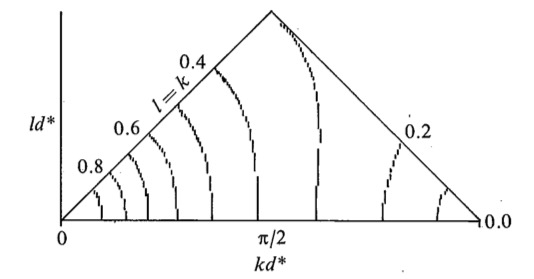
\includegraphics[keepaspectratio]{./pictest/pic461.jpg}}
% \caption{}
% \end{figure}

The wave number region in the figure is the same as in the earlier
diagrams, Figs. 2.3 and 4.1. Comparing the isolines of the present
figure with those of Fig. 2.3, where the effect of space differenc­ing
alone was considered, shows that the effect of time differencing on
phase speed is now not negligible. Implicit time differencing is seen to
result in a considerable retarda­tion of gravity waves of the same order
of magnitude as that due to centered space differencing.

To apply an implicit method it is necessary to solve the difference
system for variables at level n + 1.

With an ordinary oscillation equation, \texttt{h2.7} in
\texttt{Chapter2}, this can be done very simply. For the system
\texttt{b6.1} it is more complex. The quantities \(\delta_{x}u^{n + 1}\)
and \(\delta_{y}v^{n + 1}\) can be eliminated from the third equation by
applying operators \(\delta_{x}\) and \(\delta_{y}\) to the first and
second of these equa­tions and substituting the results into the third
equation. This gives an equation for the height which can be solved
using a number of standard methods : the most popular of these is the
\emph{relaxation method} which is discussed later in this section.

Two methods are used to deal with the advection, Coriolis, and other
terms of the governing equations, in atmospheric models. One of these,
the \emph{splitting method}, will be discussed in the next section. The
other is the semi-implicit method. There is no advantage in using an
implicit method for these additional terms of the governing equations.
They are associated with slower phase speeds, and should not require
excessively small time steps for linear stability when calculated
explicitly. Thus, they can be calculated by an explicit scheme. Since
the trapezoidal implicit scheme is a two level scheme like the
forward-backward scheme, it is convenient to use the Adams-Bashforth
scheme for this purpose. Robert (1969) in a spectral model, and
subsequently Kwizak and Robert (1971) in a grid point model, chose,
however, to use the leapfrog scheme. We then need variables at the
middle of the time step used for the implicit differencing, and,
therefore, it has to be performed over a time interval of \(2\Delta t\).
However, the scheme is now less economical for gravity waves since these
steps have to be made separately for each of the two time levels stored
in the leapfrog scheme. In return, we have a differencing for the
advection and other additional terms that is neutral and more accurate
than Adams-Bashforth\textquotesingle s. Kwizak and Robert call this
combined scheme the \emph{semi-implicit} scheme. It has been used for a
number of years in the Canadian operational model, and is becoming
increasingly popular in some other operational numerical prediction
centres.

The usual procedure used for solving the semi-implicit difference system
for variables at time level \(n + 1\) will be illustrated for the
shallow water equations. These equations can be written in a compact
form

{\[\frac{\partial u}{\partial t} = - g\frac{\partial h}{\partial x} + A_{u}\]\[\frac{\partial v}{\partial t} = - g\frac{\partial h}{\partial y} + A_{v}\]\[\frac{\partial h}{\partial t} = - H\nabla\textbf{v} + A_{h}\]}

where \(A_{u}\), \(A_{v}\) and \(A_{h}\) denote the terms that were
omitted in the system \texttt{b4.8} describing the propagation of pure
gravity waves.

When we use leapfrog differencing for these additional terms, and
implicit differencing over a time interval \(2\Delta t\) for the gravity
wave terms and centered space differencing, \texttt{b6.6} is replaced by

{\[u^{n + 1} = u^{n - 1} - g\Delta t\left( \delta_{x}h^{n - 1} + \delta_{x}h^{n + 1} \right) + 2\Delta t A_{u}^{n},\]\[v^{n + 1} = v^{n - 1} - g\Delta t\left( \delta_{y}h^{n - 1} + \delta_{y}h^{n + 1} \right) + 2\Delta t A_{v}^{n},\]\[h^{n + 1} = h^{n - 1} - H\Delta t\left[ \left( \delta_{x}u + \delta_{y}v \right)^{n - 1} + \left( \delta_{x}u + \delta_{y}v \right)^{n + 1} \right] +  2\Delta t A_{h}^{n}\]}

We now apply the operator \(\delta_{x}\) to the first, and
\(\delta_{y}\) to the second of these equations, respectively, and add
the results. We introduce the notation

\[\delta_{xx}h = \delta_x(\delta_x h ) \qquad  \delta_{yy}h = \delta_y(\delta_y h )\]

We obtain

\[\left( \delta_{x}u + \delta_{y}v \right)^{n + 1} =
\left( \delta_{x}u + \delta_{y}v \right)^{n - 1} 
- g\Delta t \left[ ( \delta_{xx} + \delta_{yy} )h^{n - 1} 
+ ( \delta_{xx} + \delta_{yy} )h^{n + 1}\right] +
2\Delta t( \delta_{x}A_{u} + {\delta_{y}A}_{v})^{n}\]

Substituting the right-hand side into the third of \texttt{b6.7}, and
defining the "finite difference Laplacian" by

\[\mathbf{\nabla_d}^2 \equiv ( \delta_{xx} + \delta_{yy} )h,\]

we find

\[\text{  h}^{n + 1} = h^{n - 1} - 2H\Delta t\left( \delta_{x}u + \delta_{y}v \right)^{n + 1}
 + gH\left( \Delta t \right)^{2}\left( \mathbf{\nabla_d}{2}h^{n - 1} + \mathbf{\nabla_d}^{2}h^{n + 1} \right) 
 + 2\Delta t\left\lbrack A_{h} - H\Delta t\left( {\delta_{x}A}_{u} + {\delta_{y}A}_{v} \right) \right\rbrack\]

Using, in addition, the definitions

\[F^{n + 1} \equiv h^{n + 1} - 2H\Delta t \left( \delta_{x}u + \delta_{y}v \right)^{n + 1} + gH(\Delta t)^{2}\mathbf{\nabla_d}^2 h^{n + 1},\]\[G^{n} \equiv 2\Delta t \left\lbrack A_{h} - H\Delta t\left( {\delta_{x}A}_{u} + {\delta_{y}A}_{v} \right) \right\rbrack^{n}\]

this can be written as

{\[h^{n + 1} - gH(\Delta t )^{2}\mathbf{\nabla_d}^{2}h^{n + 1} = F^{n + 1} + G^{n}\]}

The terms have been arranged to show that at time level n the right-hand
side is known at all space grid points. Once this equation has been
solved for the values \(h^{n + 1}\), \(u^{n + 1}\) and \(v^{n + 1}\) can
be obtained directly from the first and second of \texttt{b6.7}. We now
consider ways of solving \texttt{b6.8}.

The quantity \(\mathbf{\nabla_d}^{2}h\) on the left side of
\texttt{b6.8} is an approxi­mation to \(\nabla^{2}h\). Using the
notation of \texttt{figg:462}, it can be written as

% \begin{figure}
% \centering
% \pandocbounded{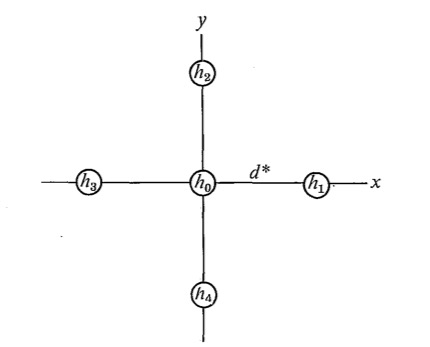
\includegraphics[keepaspectratio]{./pictest/pic462.jpg}}
% \caption{}
% \end{figure}

{\[\mathbf{\nabla_d}^2 h = \frac{1}{4(d^*)^2}\left( h_{1} + h_{2} + h_{3} + h_{4} - 4h_{0} \right)\]}

Thus, \texttt{b6.8} is a finite difference approximation to an elliptic
equation

\[\nabla^{2}h + ah + b\left( x,y \right) = 0\]

To solve such an equation, it is necessary to know the values of
\(h(x,y)\) at the boundaries of the computation region. For a numerical
solution we write \texttt{b6.8} at each of the interior grid points
where the variable h is carried. In this way we obtain a system with one
equation for each interior grid point. There is one unknown for each
grid point. In each of the equations, except the equations for points
adjacent to the boundary, there are five of these unknowns. There are no
difficulties in principle in solving such a system of linear equations,
but, since the number of equations is normally exceedingly large, of the
order of 1000 or more, it is not obvious how to set about it.

The method usually used is the relaxation method. This consists of the
following steps.

a) An arbitrary guess is made for the field \(h^{n + 1}\). Usually the
field of the preceding time step, \(h^{n}\), is taken as this first
guess.

b) At each of the grid points the value \(h^{n + 1}\) is changed so as
to satisfy the difference equation, in our case \texttt{b6.8}. These
changes can be made simultaneously at all grid points (simultaneous or
Richardson relaxation), or sequen­tially, point by point (sequential
oxLiebmann relaxation).

c) The preceding step is repeated as many times as needed to make the
change at every point less than some preassigned small value.

The relaxation method always converges. Experience shows that the
convergence is faster for sequential relaxa­tion, and also if the
changes calculated to satisfy the equation exactly are multiplied by a
factor having a value between 1 and 2 (overrelaxation factor) before
being added on. For a particular problem the optimum value of this
overrelaxation factor can easily be found by numerical experiments, in
which the number of iterations required is plotted as a function of the
value of the overrelaxation factor. This optimum value can be shown to
be not much less than 2. More details on the relaxation method can be
found in textbooks by Thompson (1961) and by Haltiner (1971).

The algebraic system given by equations of the type \texttt{b6.8} can
also be solved by \emph{direct methods} (e.g. Kreiss and Oliger, 1973,
p. 54). Direct method can be more efficient than the relaxation
procedure ; thus, they are typically used when relaxation requires very
large compu­tation time, as may happen, for example, in convection
studies. When implicit schemes are used for simulation or prediction of
large scale atmospheric motions, the time needed for relaxation is
several times less than the time needed for other steps of the
integration procedure, so that only a small fraction of the total
computer time can be saved by using a faster direct method. For that
reason the use of direct methods, requiring a larger programming effort,
is not popular in these models.

Generalization to the three-dimensional case of the procedure for
solving the semi-implicit system for variables at level \(n + 1\)
outlined here is not quite trivial. The reader is referred to the paper
by Robert \emph{et al}. (1972).

Implicit schemes were first used extensively in atmo­spheric models by
Marchuk (Marchuk, 1967). With the semi-implicit scheme it is also
possible to construct an economical grid analogous to the Eliassen grid
for the leapfrog scheme ; the appropriate space-time stagger­ing of the
variables was pointed out by Gerrity and McPherson (1971). A
semi-implicit scheme somewhat different from the one outlined here has
been developed by Burridge, and is now used in the British operational
model (Burridge and Hayes, 1974). Implicit and semi-implicit schemes are
undoubtedly the most efficient schemes used in atmospheric models. To
achieve this economy we have to put additional effort into solving an
elliptic equation. Furthermore they are associated with an appreciable
deceleration of gravity waves. Thus, the implicit schemes do not seem
suitable for the study of details of the geostrophic adjustement
process. How­ever, this deceleration does not appear particularly
harmful for the simulation and prediction of the large-scale
quasi-geostrophic motions. For example, Kwizak and Robert (1971) have
found that barotropic 5-day forecasts made with explicit differencing
and time steps of 10 min are almost identical to those made with
semi-implicit differencing and time steps of 60 min. Later Robert et al.
(1972) have calculated the differences be­tween 5-day forecasts obtained
using 30 and 60 min time steps for a baroclinic 5-leveI semi-implicit
model. These differences were found to be insignificant compared to
other sources of error normally present in numerical models. However,
the model used for these experiments did not include topography, surface
friction, and other physical processes ; one might expect the
deceleration of gravity waves to have a more noticeable effect when
these physical processes (e.g. the release of latent heat) are present,
since then the gravity waves should be more significant. On the other
hand, the computation time saved by the implicit differencing can be
used to reduce the grid size on the computation. This would decrease the
phase speed error for all the waves, including the gravity waves.

\subsection{\texorpdfstring{\textbf{The splitting or Marchuk
method}}{The splitting or Marchuk method}}\label{the-splitting-or-marchuk-method}

The complexity of the system of hydrodynamic equa­tions, that is, the
simultaneous presence of a number of physical factors, may cause some
difficulties. One difficulty was mentioned in the preceding section : if
we wanted to approximate \texttt{b6.6} using a fully implicit scheme we
would obtain a system for the variables at level that is practically
impossible to solve. Also since different physical factors are present
in this system we will nor­mally wish to use different schemes for terms
associated with them. Thus, considering the linearized system with
advection and gravity wave terms,

{\[\frac{\partial u}{\partial t} + c\frac{\partial u}{\partial x} + g\frac{\partial h}{\partial x} &= 0\]\[\frac{\partial h}{\partial t} + c\frac{\partial h}{\partial x} + H\frac{\partial u}{\partial x} &= 0\]}

we might wish to use one scheme for the advection terms, and another for
the gravity wave terms — in much the same way as was done within the
semi-implicit scheme. In such a situation, even though both of the
schemes to be used are stable considered one at a time, we cannot be
certain that the scheme obtained as a combination of the two will also
be stable. An example where it is not was given by Kasahara (1965).

These problems can be avoided by using the \emph{splitting method}. The
idea of this method is to construct schemes for a complex system of
equations so that \emph{within each time step} this system is split into
a number of simpler subsystems, which are then solved consecutively one
at

a time. In the case of \texttt{b7.1}, within a given time step, we could
first solve the system of advection equations

{\[\frac{\partial u}{\partial t} + c\frac{\partial u}{\partial x} = 0\]\[\frac{\partial h}{\partial t} + c\frac{\partial h}{\partial x} = 0\]}

Denote the provisional values \(u^{n + 1}, h^{n + 1}\) obtained in this
way by \(u^{*},h^{*}\). Use these values at the beginning of the time
step for solving the remaining subsystem

{\[\frac{\partial u}{\partial t} + g\frac{\partial h}{\partial x} = 0\]\[\frac{\partial h}{\partial t} + H\frac{\partial u}{\partial x} = 0\]}

The values \(u^{n + 1}\), \(h^{n + 1}\), obtained after solving also
this other subsystem, are now taken as actual approximate values of
these variables at the level \(n + 1\). The procedure is repeated in
each following time step.

A solution obtained by the splitting method will repre­sent a consistent
approximation to the true solution. This can be proved easily for a
particular choice of schemes for solving the subsystems. The approximate
values of the dependent variables then have to approach the true values
as the time step approaches zero.

To study the stability of schemes constructed by the splitting method,
we consider the example above. Denote by \(\lambda_{a}\) and
\(\lambda_{b}\) the values of \(\lambda\) of the schemes chosen for the
numerical solution of subsystems \texttt{b7.2} and \texttt{b7.3},
respectively. Then, we have

\[u^{*} &= Re\left( \lambda_{a}\lambda^{n}\widehat{u}e^{ikx} \right)\]\[h^{*} &= Re\left( \lambda_{a}\lambda^{n}\widehat{\lambda}e^{ikx} \right)\]

and

\[u^{n + 1} = Re\left( \lambda_{b}\lambda_{a}\lambda^{n}\widehat{u}e^{\text{ikx}} \right)\]\[h^{n + 1} = Re\left( \lambda_{b}\lambda_{a}\lambda^{n}\widehat{u}e^{\text{ikx}} \right)\]

Therefore, we find,

\[\lambda = \lambda_{b}\lambda_{a}\]

and

\[\left| \lambda \right| = \left| \lambda_{b} \right|\left| \lambda_{a} \right|\]

Thus, if both of the schemes chosen for the solution of subsystems
\texttt{b7.2} and \texttt{b7.3} are stable, the combined scheme
constructed by the splitting method will also be stable. This conclusion
can be generalized for an arbi­trary system of equations and number of
subsystems.

When applying the splitting method, we do not neces­sarily have to use
equal time steps for each of the subsys-This may well be the main
advantage of the splitting method : we can choose a relatively long time
step for the subsystem governing a slow process, advection in the
present example, and then use a number of smaller steps to calculate the
faster process. Since the advection process is the most expensive in
computation time within the primitive equations, significant economies
can be accomplished in this way. A disadvantage of the method is that
calculation of the effects of different physical factors one at a time
usually leads to an increase in the truncation error. For example,
Burridge and Hayes (1974) suggest that the technique of splitting the
governing equations into advection and adjustment stages does not allow
time steps longer than 12 to 15 min if the time-truncation is not to
become significant.

The splitting method was first used in atmospheric models by Marchuk
(Marchuk, 1967); thus, in mete­orology it is also known as the
\emph{Marchuk method}. It would appear that the splitting method is used
for most atmospheric models in the Soviet Union. The splitting technique
is used also in the British operational model (Burridge and Hayes,
1974), and in a limited area model by Lepas and his collaborators (Lepas
et al., 1974).

\subsection{\texorpdfstring{\textbf{Two-grid-interval
noise}}{Two-grid-interval noise}}\label{Section4.8}

Unless we are using the lattice (C) shown in \texttt{figg:421} we will
always have a problem with two-grid-interval waves. These are false
stationary waves appearing as neutral solutions of the difference
equations for gravity waves. When the Coriolis terms are also present,
as seen in Section \texttt{Section4.3}, the two-grid-interval waves
appear with false low frequencies as pure inertia waves, or, with
lattice (D), as stationary waves.

A number of methods have been used to cope with this. In many models
dissipative schemes are used to give maximum damping for the
two-grid-interval wave, or lateral diffusion is added with relatively
large diffusion coefficients. The appearance of excessive
two-grid-interval noise is thereby suppressed. However, instead of
attacking the \emph{consequences} of inadequacies in a simula­tion of a
physical process, it is generally better to look for a method that would
achieve a physically correct simulation of that process, and thus
eliminate the cause of the difficulty, One method this kind for dealing
with the two-grid-interval wave problem has been suggested and used by
Arakawa (1972). It consists of an intermittent use of uncentered space
differencing within the gravity wave terms, performed alternately on
opposite sides of the central point.

Mesinger (1973) showed how two-grid-interval wave noise could be
prevented in some cases even by using cen­tered differencing; this
method will be outlined briefly here. We consider the system of
linearized gravity wave equations

{\[\frac{\partial u}{\partial t} + g\frac{\partial h}{\partial x} &= 0\]\[\frac{\partial v}{\partial t} + g\frac{\partial h}{\partial y} &= 0\]\[\frac{\partial h}{\partial t} + H\nabla\cdot\mathbf{v} &= 0\]}

Consider any two neighbouring height points for example within the
lattice (E). A height perturbation at one of these points cannot affect
the other point because there is no velocity point in between ; this
velocity is needed to cause a height change at the other point through
the divergence term in the continuity equation. To circum­vent this
difficulty we can introduce auxiliary velocity points midway between the
height points. Velocity components at these auxiliary points can be
assumed equal to an average of velocities at the two neighbouring
velocity points at the beginning of a time step, and the acceleration
contributions can then be evaluated and added to these initial values to
obtain components at the middle or at the end of the time step. Only the
velocity components and accelerations along directions joining the two
height points are needed, and these accelerations can be calcu­lated
using the height values at the two points. The resulting velocity
components can then be used for a more accurate calculation of the
divergence term in the conti­nuity equation. In this way schemes are
obtained in which a height perturbation at a single grid point is
propagated by gravity waves to all the other height grid points.
Therefore there can be no grid-splitting and two grid-interval noise in
the height field. Since a velocity perturbation can propagate as a
gravity wave only by exciting height perturbations, the procedure will
prevent false two-grid-interval noise in all the variables.

We shall illustrate this procedure using the implicit scheme,
\texttt{b6.1}. The velocity components at regular velocity points are
computed in the same way as before, so the first two equations of that
system remain unchanged. To calculate the velocity divergence in the
continuity equation we define auxiliary velocity points midway between
the neighbouring height points, as shown by the circled numbers 5, 6, 7
and 8 in \texttt{figg:481}. Using the system \(x^{'},y^{'}\) shown in
this figure, components \(u\) are needed at points 5 and 7, and
components v\textquotesingle{} at points 6 and 8.

At the beginning of the time step \(\Delta t\) these components are
obtained by

% \begin{figure}
% \centering
% \pandocbounded{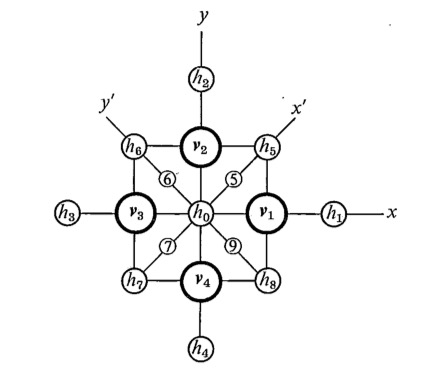
\includegraphics[keepaspectratio]{./pictest/pic481.jpg}}
% \caption{}
% \end{figure}

space-averaging, that is

\[u^{'n} &= \frac{\sqrt{2}}{2}\left( {\overline{u}}^{y'} + {\overline{v}}^{y'} \right)^{n},\]\[v^{'n} &= \frac{\sqrt{2}}{2}\left( - {\overline{u}}^{x'} + {\overline{v}}^{x'} \right)^{n}.\]

An overbar denotes a two-point average taken along the direction
indicated following the bar sign. Acceleration contributions are added
to these initial values to obtain values at the end of the time step,

\[u^{'n + 1} &= u^{'n} - g\Delta t\frac{1}{2}\left( \delta_{x'}h^{n} + \delta_{x'}h^{n + 1} \right)\]\[v^{'n + 1} &= v^{'n} - g\Delta t\frac{1}{2}\left( \delta_{y'}h^{n} + \delta_{y'}h^{n + 1} \right)\]

The velocity divergence in the continuity equation can now be
approximated by

\[\frac{1}{2}\left( \delta_{x}u + \delta_{y}v \right) + \frac{1}{2}\left( \delta_{x}u^{'} + \delta_{y}v^{'} \right)\]

giving equal weight to all eight directions of the lattice. In this way
the implicit approximation to the continuity equation may be obtained as

{\[h^{n + 1} = h^{n} - H\Delta t\left( \delta_{x}u + \delta_{y}v \right)^{n} 
+ \frac{1}{4}gH( \Delta t)^{2}\left( \nabla_{0}^{2}h^{n} + \nabla_{0}^{2}h^{n + 1} \right)\]}

Here the velocity components at level \emph{n + 1} have already been
eliminated using the first two of \texttt{b6.1}, and

{\[\nabla_{0}^{2} \equiv \frac{1}{4d^{2}} \times \left[ h_{1} + h_{2} + h_{3} + h_{4} + 2\left( h_{5} + h_{6} + h_{7} + h_{8} \right) - 12h_{0} \right]\]}

This is again a finite difference approximation to \(\nabla^{2}h\), but
now it is calculated using the height values of nine neigh­bouring
height points.

Comparing this scheme with the standard implicit scheme of Section
\texttt{Section4.6}, the only modification is that this nine-point
Laplacian has replaced the five-point Laplacian \texttt{b6.9} in the
continuity equation. This allows propagation of gravity waves between
all height points of the grid, thus admitting no false space noise in
the height field. A more detailed analysis of the properties of the
scheme can be found in Mesinger (1973). The modification, for example,
has no effect on the uncondi­tional stability of the implicit scheme ;
however, instead of being neutral for all waves, the scheme now damps
shorter waves to some extent. The modified scheme has a smaller
truncation error than the unmodified scheme.

Analogous modifications of some other schemes have been discussed in
papers by Janjic (1974) and Mesinger (1974). All of these papers show
that the modified schemes are strikingly superior in the case of a
stationary circular vortex, forced at a single height grid point. A note
by Mesinger and Janjic (1974) provides, further­more, a dramatic
illustration of the advantages of the proposed method in the case of a
limited area model, requiring lateral boundary conditions to be
prescribed. In a 5-level model using the unmodified forward-back­ward
scheme, intense short-wave noise was generated at the boundaries of the
region, a problem noticed also by earlier investigators (e.g. Miller
\emph{et al}., 1972 ; Krishnamurti et al., 1973). With the scheme
modified along these lines, however, there were no difficulties due to
the prescribed boundary conditions, even with no lateral diffusion in
the model.

It is important to be aware that this method is not attempting to
improve the calculation of short gravity waves of wave lengths close to
two grid intervals. At this scale the finite difference representation
is very poor, and significant improvements in accuracy can hardly be
expected. The problem is that gravity waves, with longer wave lengths
can propagate independently on individual (C) type subgrids, and thus
erroneously appear to have wave lengths close to two grid intervals.
Thus, we are confronted with a kind of aliasing error. The proposed
method enables these waves to appear with wave lengths close to their
physical value instead in the noise region with wave lengths close to
two grid intervals.

\subsection{\texorpdfstring{\textbf{Time noise and time
filtering}}{Time noise and time filtering}}\label{time-noise-and-time-filtering}

In addition to the appearance of spurious short-wave noise in space,
spurious short-wave noise in time, that is, high frequency noise can
appear in numerical models.

One mechanism causing this when the leapfrog scheme is used for
nonlinear equations is the separation of solutions at alternate time
steps, generating two-grid-interval noise in time. Such separation is
illustrated in a paper by Lilly (1965, p. 23).

High frequency noise appears in atmospheric models also as a result of
difficulties in observing initial condi­tions representative of the
large scale atmospheric motions. The observed initial conditions contain
instru­mental errors, are influenced by meso and small scale motions,
are not known at grid points of the model, and, finally, are completely
absent over relatively large areas of the globe. As a result of all of
these factors, if initial grid point values are interpolated directly
from the observed data the numerical forecasts will contain spurious
gravity waves of unrealistically large amplitudes.

In the early successful integrations of the primitive equations these
problems were partially by-passed by obtaining the initial winds from
the initial geopotential fields as a solution of the \emph{balance
equation} — the equation obtained by assuming the initial velocity
divergence and its time derivative to be equal to zero. Initial
conditions prepared in this way (e.g. Haltiner, 1971) prevent exces­sive
high-frequency gravity wave noise.

It is now generally accepted that this is not the best way of preparing
the initial conditions. First, the wind data are not used when solving
the balance equation, and some information is lost. It has also been
shown (e.g. Phillips, 1960b ;Winninghoff, 1968) that the presence of a
realistic initial divergent wind field should have a beneficial effect
on the forecast, Finally, an increasing fraction of the observations are
now continuous, and in time not obtained at specific times. The methods
being used to extract the maximum information from this type of data
rely more on running a prediction model to adjust the data in space and
time (e.g. Bengtsson, 1975). In such an integration relatively intense
high frequency noise is generated.

The first of the mechanisms mentioned here, separation of solutions at
alternate time steps, has to be suppressed in some way — otherwise it
may lead to a complete breakdown of the integration. One method that is
used for this purpose is an intermittent step made with a two level
scheme. A weakness of such a procedure is that the choice of the
solution that is eliminated is arbi­trary.

Experience shows that the noise generated by assi­milation of the
observed data typically dies out to an acceptable level in about 24
hours of simulated time due to geostrophic adjustment. However, it may
be desirable to accelerate this adjustment by appropriate numerical
techniques. The Matsuno scheme can be used for this purpose.

Another method that can be used to increase the damping of high
frequency noise in atmospheric models is \emph{time filtering}
originally proposed by Roberts (1966). To apply this at least three
consecutive values of the function to be filtered are needed. We shall
consider the simplest case where this minimum number of three values is
used. It suffices to consider one function only, which we assume to be a
solution of the oscillation equation. Thus, we consider the function

{\[U\left( t \right) = U\left( 0 \right)e^{i\omega t}\]}

where the values \(U\left( t - \Delta t \right)\), \(U\left( t \right)\)
and \(U\left( t + \Delta t \right)\), are known.

We shall first examine the effect of changing only the middle of these
three values using the relation

{\[\overline{U(t)} = U(t) + \frac{1}{2}S  \left[ U\left( t - \Delta t \right) - 2U\left( t \right) + U\left( t + \Delta t \right) \right]\]}

known as the \emph{centered filter}. The overbar now denotes the
filtered value of a function, and \(S\) is the \emph{filter parameter}.
The expression within the square bracket in \texttt{b9.2} is
pro­portional to the simplest approximation to the second derivative in
time ; thus, for sufficiently small positive values of \(S\) application
of the filter \texttt{b9.2} will decrease the curvature in a graph of
the three values of \(U(t)\)

For a quantitative analysis of the effect of the filter we define

{\[\overline{U(t)} \equiv R U(t)\]}

where the complex factor \(R\) is called the \emph{response} of the
filter. When this is substituted into \texttt{b9.2} and we use
\texttt{b9.1}, we obtain

{\[R = 1 - S\left( 1 - \cos{\omega\Delta t} \right)\]}

It is convenient to define \(R \equiv \left| R \right|e^{i\delta}\).

We can then say that the phase change \(\delta\) resulting from the
centered filter is zero, and that within the CFL stability criterion and
for small positive values of \(S\) the amplitude factor
\(\left| R \right|\) exerts a damping effect increasing with increasing
frequencies.

When, however, a filter is continually applied during a numerical
integration, the value \(U\left( t - \Delta t \right)\) has already been
changed prior to changing \(U(t)\). It is then appro­priate to consider
the filter

{\[\overline{U(t)} = U\left( t \right) + \frac{1}{2}S \left\lbrack \overline{U}\left( t - \Delta t \right) - 2U\left( t \right) + U\left( t + \Delta t \right) \right\rbrack\]}

Asselin (1972) calls this the basic time filter. A procedure like the
one used in deriving \texttt{b9.4} now gives

{\[R = \frac{( 2 - S )^{2} + 2S^{2}\left( 1 - \cos{\omega\Delta t} \right)}{( 2 - S^{2} ) + 4S\left( 1 - \cos{\omega\Delta t} \right)}e^{i\omega\Delta t}.\text{        }\]}

Thus, there is now a phase change that is different from zero; however,
it is small for small values of \(\omega\Delta t\). The amplitude factor
is not much different from that of the centered filter for small values
of \(S\). More details can be found in the paper by Asselin.

An analysis of the effect of the time filter for some particular choices
of time differencing schemes — the leapfrog, implicit and semi-implicit
schemes — can also be found in the paper by Asselin. We find, for
example, that the time filter in conjunction with the leapfrog scheme
can give a procedure damping the high frequencies in a more selective
way than the Matsuno scheme — less for low frequencies and more for high
frequencies. Since the computer time needed for application of the
filter is relatively small, this means that one obtains a better result
with only about half of the computer time. However, the application of
the filter does require the storage of the time dependent variables at
three time levels, that is, at one level more than with the standard
leapfrog scheme.

Using an analogous approach one can analyze the effect of smoothing and
filtering in space. The reader is referred to a review article by
Shapiro (1970) or the textbook by Haltiner (1971). It is, however, not
obvious that there are physical or computational reasons for using
two-dimensional space filtering in atmospheric models.

\subsection{\texorpdfstring{\textbf{Dissipation in numerical
schemes}}{Dissipation in numerical schemes}}\label{dissipation-in-numerical-schemes}

In concluding this chapter we add, following Arakawa (1970), a few
remarks regarding the role of dissipation that may be inherent in
numerical schemes. The discus­sion of the preceding chapter shows that
the use of dissipative schemes for the advection process should be
avoided — provided care is taken to avoid a false cascade of energy to
short waves. However, such short waves can still be generated as a
result of false reflections at boundaries on the down-stream side of the
region (Mat­suno, 1966c), or false reflections at sudden jumps in the
grid size, or at places where coefficients change rapidly. The use of
dissipative advection schemes at those places, and only at those places,
is justified.

The situation is different when we are now considering the
gravity-inertia wave terms, governing the geostrophic adjustment
process. This process is a result of the dis­persion of high frequency
waves. Use of a frequency-selective dissipative scheme will make these
high fre­quency waves damp out at a faster rate, and thus acce­lerate
the adjustment process, although the actual phy­sical process is
dispersive rather than dissipative. This gives an effect much the same
as that of time filtering. Therefore, if we are only interested in the
final result of the geostrophic adjustment process, dissipation in the
gravity-inertia wave terms may be helpful, especially when the high
frequency waves are predominantly unphysical. If we are interested in
the high frequency waves themselves, the use of a dissipative scheme
must, of course, be avoided.

\subsection{Numerical methods REFERENCES}



Ames, W. F., 1969. Numerical Methods for Partial Differential Equations.
London, Nelson. 291 pp.

Anderson, D. and Fattahi, В., 1974. A comparison of numerical solutions
of the advective equation. J. Atmos. Sci., 31, 1500-1506.

Arakawa, A., 1966. Computational design for long-term numerical
integration of the equations of fluid motion : Two dimensional
incompressible flow. Part I. J. Comput. Phys., 1, 119-143.

— 1970. Numerical simulation of large-scale atmospheric
motions.Numerical Solution of Field Problems in Continuum Physics, Proc.
Symp. Appl. Math., Durham, N. C, 1968. SIAM-AMS Proc, 2, 24-40.

— 1972. Design of the UCLA general circulation model. Numerical
Simulation of Weather and Climate, Dept. of Meteorology, Univ. of
California, Los Angeles, Tech. Rept. 7, 116 pp.

—- and Lamb, V. R., 1976. Computational design of the UCLA General
Circulation Model. To be published in Methods in Computational Physics,
Academic Press, New York.

Asselin, R., 1972.Frequency filter for time integrations. Mon. Wea.
Rev., 100, 487-490.

Bengtsson, L., 1975. 4-dimensional assimilation of meteorological
observations.WMO/ICSU Joint Organizing Committee, GARP Publications
Series No. 15, 76 pp.

Bjerknes, V., 1904. Das Problem der Wettervorhersage,
betrachtetvomStandpunkte der Mechanik und der Phvsik. Meteor.
Zeit-schr., 21, 1-7.

Burridge, D. M. and Hayes, F. R., 1974. Development of the British
operational model. The GARP Programme on Numerical Experimentation,
Rept. 4, 102-104.

Charney, J. G., 1966. Some remaining problems in numerical weather
prediction.Advances in Numerical Weather Predic­tion, Hartford, Conn.,
Travelers Research Center, Inc., 61-70.

—, Fjortoft, R. and von Neumann, J., 1950. Numerical integration of the
barotropicvorticity equation.Tellus, 2, 237-254.

Courant, R., Friedrichs, K. and Lewy, H., 1928.
UberdiepartiellenDifferenzengleichungen der mathematischenPhysik. Math.
Annalen, 100, 32-74.

— and Hilbert, D., 1953. Methods of Mathematical Physics, Vol. I. New
York, Interscience. 562 pp.

Cullen, M. J. P., 1974. Integration of the primitive equations on a
sphere using the finite element method. Quart. J. Roy. Meteor. Soc, 100,
555-562.

Deardorff, J. W., 1974. Three-dimensional numerical study of the height
and mean structure of a heated planetary boundary layer. Boundary-Layer
Meteor.,7, 81-106.

Egger, J., 1971. Mindestgrösse von Gebirgen und Konvektions-gebieten,
die in den Modellen der numerischen Vorhersage berück­sichtigt werden
können. Beitr. Phys. Atmos., 44, 245-271.

Eliassen, A., 1956. A procedure for numerical integration of the
primitive equations of the two-parameter model of the atmosphere.
Large-Scale Synoptic Processes, Dept. of Meteorology, Univ. of
California, Los Angeles, Sci. Rept. 4, 53 pp.

Fischer, G., 1959. Ein numerisches Verfahren zur Errechnung von Windstau
und Gezeiten in Randmeeren. Tellus, 11, 60-76.

Fjortoft, R., 1953. On the changes in the spectral distribution of
kinetic energy for two-dimensional, nondivergentflow.Tellus5 225-230.

Gadd, A. J., 1974a.An economical explicit integration scheme.
Meteorological Office Tech. Note 44, 7 pp.

— 1974b. Fourth order advection schemes for the 10 level model.
Meteorological Office Tech. Note 45, 8 pp.

Gerrity, J. P., Jr. and McPherson, R. D., 1971. On an efficient scheme
for the numerical integration of a primitive-equation barotropic model,
i. Appl. Meteor.,10, 353-363.

Haltiner, G. J., 1971. Numerical Weather Prediction.New York Wiley, 317
pp.

Harlow, F. H. and Amsden, A.A., 1971. Fluid dynamics. Los Alamos
Scientific Laboratory of the Univ. of California, Mono­graph LA-4700,
115 pp.

Hinkelmann, K., 1959. Ein numerisches Experiment mit den primi­tiven
Gleichungen. The Atmosphere and the Sea in Motion, Rossby Memorial
Volume, New York, Rockefeiler Institute Press, 486-500.

Janjic, Z. I., 1974. A stable centered difference scheme free of
two-grid interval noise. Mon. Wea. Rev., 102, 319-323.

Jespersen, D. C, 1974.Arakawa\textquotesingle s method is a
finite-element method. J. Comput. Phys., 16, 383-390.

Kasahara, A., 1965.On certain finite-difference methods for fluid
dynamics. Mon. Wea. Rev., 93, 27-31.

— 1969. Simulation of the earth\textquotesingle s atmosphere. National
Center for Atmospheric Research, Boulder, Colo., NCAR Manuscript 69-27,
42 pp.

FCreiss, H. and Öliger J., 1973.Methods for the approximate solution of
time dependent problems.WMO/ICSU Joint Organizing Committee, GARP
Publications Series No. 10, 107 pp.

Krishnamurti, T. N., Kanamitsu, M., Ceselski, B. and Mathur, M. B.,
1973.Florida State University\textquotesingle s Tropical Prediction
Model.Tellus, 25, 523-535.

Kurihara, Y., 1965. On the use of implicit and iterative methods for the
time integration of the wave equation. Mon. Wea. Rev., 93, 33\^{}t6.

90

THE GRAVITY AND GRAVITY-INERTIA WAVE EQUATIONS

Kwizak, M. and Robert, A. J., 1971. A semi-implicit scheme for grid
point atmospheric models of the primitive equations. Mon. Wea. Rev., 99,
32-36.

Lax, P. D. and Wendroff, B., 1960. Systems of conservation laws.Commun.
Pure Appl. Math., 13, 217-237.

Leith, C., 1965.Lagrangian advection in an atmospheric model.WMO-IUGG
Symposium on Research and Development Aspects of Long Range Forecasting,
Boulder, Colo., 1964. WMO Tech. Note 66, 168-176.

Lepas, J., Benlareche, M., Coiffier, J., Finke, L. and Tagnit-Hammou,
A., 1974.Primitive equations model — implicit method for numerical
integration. The GARP Programme on Numerical Experimentation, Rept. 4,
65.

Lilly, D. K., 1965.On the computational stability of numerical solutions
of time-dependent non-linear geophysical fluid dynamics problems. Mon.
Wea. Rev., 93, 11-26.

Matsuno, T., 1966a. Numerical integrations of the primitive equa­tions
by a simulated backward difference method. J. Meteor. Soc. Japan, Ser.
2, 44, 76-84.

— 1966b. A finite difference scheme for time integrations of
oscilla­tory equations with second order accuracy and sharp cut-off for
high frequencies. J. Meteor. Soc. Japan, Ser. 2, 44, 85-88.

— 1966c. False reflection of waves at the boundary due to the use of
finite differences. J. Meteor. Soc. Japan, Ser. 2, 44, 145-157.

Mesinger, F., 1971. Numerical integration of the primitive equations
with a floating set of computation points : Experiments with a
barotropic global model. Mon. Wea. Rev., 99, 15-29.

— 1973. A method for construction of second-order accuracy differ­ence
schemes permitting no false two-grid-interval wave in the height
field.Tellus, 25, 444-458.

— 1974. An economical explicit scheme which inherently prevents the
false two-grid-interval wave in the forecast fields. Difference and
Spectral Methods for Atmosphere and Ocean Dynamics Problems, Proc.
Symp., Novosibirsk, 1973, Part II, 18-34.

— andJanjic Z. I., 1974. Noise due to time-dependent boundary conditions
in limited area models. The GARP Programme on Numerical Experimentation,
Rept. 4, 31-32.

Miller, B.I., Chase, P.P. and Jarvinen, B. R., 1972. Numerical
prediction of tropical weather systems. Mon. Wea. Rev., 100, 825-835.

Orszag, S. A., 1971. On the elimination of aliasing in finite-difference
schemes by filtering high-wavenumber components. J. Atmos. Sci., 28,
1074.

Phillips, N. A., 1956. The general circulation of the atmosphere : a
numerical experiment. Quart. J. Roy. Meteor. Soc, 82, 123-164.

— 1959. An example of non-linear computational instability. The
Atmosphere and the Sea in Motion, Rossby Memorial Volume, New York,
Rockefeller Institute Press, 501-504.

— 1960a. Numerical weather prediction.Advances in Computers, New York,
Academic Press, 1, 43-90.

— 1960b. On the problem of initial data for the primitive
equations.Tellus, 12, 121-126.

Platzman, G. W., 1958 .The lattice structure of the finite-difference
primitive and vorticity equations. Mon. Wea. Rev., 86, 285-292.

— 1963. The dynamical prediction of wind tides on Lake Erie. Meteor.
Monogr., 4, No. 26, 44 pp.

— 1964. An exact integral of complete spectral equations for un­steady
one-dimensional flow. Dynamical Prediction Group, Dept. of the
Geophysical Sciences, Univ. of Chicago, Tech. Rept. 16, 28 pp.

Richardson, L. F., 1922. Weather Prediction by Numerical Process.
London, Cambridge University Press/reprinted: Dover, 1965/. 236 pp.

Richtmyer, R. D., 1963. A survey of difference methods for non-steady
fluid dynamics. National Center for Atmospheric Research, Boulder,
Colo., NCAR Tech. Notes 63-2, 25 pp.

— and Morton, K. W., 1967. Difference Methods for Initial Value
Problems. New York, Interscience. 406 pp.

Robert, A. J., 1966. The integration of a low order spectral form of the
primitive meteorological equations. J. Meteor. Soc. Japan, Ser. 2, 44,
237-245.

— 1969. The integration of a spectral model of the atmosphere by the
implicit method.Proc. WMO/IUGG Symposium on Numerical Weather Prediction
in Tokyo, 1968. Meteor. Soc. Japan. VII-19-VII-24.

—, Henderson, J. and Turnbull, C, 1972. An implicit time integra­tion
scheme for baroclinic models of the atmosphere. Mon. Wea. Rev., 100,
329-335.

— 1974. Computational resolution requirements for accurate medium-range
numerical predictions. Difference and Spectral Methods for Atmosphere
and Ocean Dynamics Problems, Proc. Symp., Novosibirsk, 1973, Part I,
82-102.

Sawyer, J. S., 1972.Numerical weather prediction within World Weather
Watch — past, present and future.Tenth Anniversary of the World Weather
Watch, Geneva, WMO Publ. No. 342, 33-44.

Shapiro, R., 1970.Smoothing, filtering, and boundary effects. Rev.
Geophys. Space Phys., 8, 359-387.

Shuman, F. G., 1974. Analysis and experiment in nonlinear computa­tional
stability. Difference and Spectral Methods for Atmosphere and Ocean
Dynamics Problems, Proc. Symp., Novosibirsk, Part I, 51-81.

—, Brown, J. A. and Campana, K., 1975. A new explicit differencing
system for primitive equations.In preparation.

Sielecki, A., 1968.An energy-conserving difference scheme for the storm
surge equations. Mon. Wea. Rev., 96, 150-156.

Thompson, P. D., 1961. Numerical Weather Analysis and Prediction. New
York, Macmillan. 170 pp.

Winninghoff, F. J., 1968. On the adjustment toward a geostrophic balance
in a simple primitive equation model with application to the problems of
initialization and objective analysis.Ph. D. thesis, Dept. of
Meteorology, Univ. of California, Los Angeles, 161 pp.

Wurtele, M. G., 1961. On the problem of truncation error.Tellus, 13,
379-391.

Young, J. A., 1968. Comparative properties of some time differencing
schemes for linear and non-linear oscillations. Mon. Wea. Rev., 96,
357-364.

GARP PUBLICATIONS SERIES

No. 1 An Introduction to GARP

No. 2 COSPAR Working Group VI Report to JOC — Systems Possibilities for
an Early GARP Experiment (out of print)

No. 3 The Planning of the First GARP Global Experiment (out of print)

No. 4 The Planning of GARP Tropical Experiments (out of print)

No. 5 Problems of Atmospheric Radiation in GARP

No. 6 Numerical Experimentation Related to GARP

No. 7 The GARP Programme on Numerical Experimentation

No. 8 Parameterization of Sub-Grid Scale Processes

No. 9 The Basic Data Set Project

No. 10 Methods for the Approximate Solution of Time-Dependent Problems

No. 11 The First GARP Global Experiment — Objectives and Plans

No. 12 The Complete Atmospheric Energetics Experiment (CAENEX)

No. 13 The Air Mass Transformation Experiment (AMTEX)

No. 14 Modelling for the First GARP Global Experiment

No. 15 Four-Dimensional Assimilation of Meteorological Observations

No. 16 The Physical Basis of Climate and Climate Modelling

No. 17 Numerical Methods Used in Atmospheric Models

No. 18 The Monsoon Experiment (MONEX)

GARP SPECIAL REPORTS

No. 1 Report of Planning Conference on GARP — Brussels, March 1970

No. 2 Report of Interim Planning Group on GARP Tropical Experiment in
the Atlantic — London, July 1970

No. 3 Report of the First Session of the Tropical Experiment Council —
Geneva, February 1971

No. 4 Report of the First Session of the Tropical Experiment Board —
Geneva, February 1971

No. 5 Report of the Second Session of the Tropical Experiment Board —
Geneva, December 1971

No. 6 Report of the Third Session of the Tropical Experiment Board —
Geneva, April 1972 (out of print)

No. 7 Report of the Second Session of the Tropical Experiment Council —
Geneva, September 1972

No. 8 Report of the Planning Conference on the First GARP Global
Experiment — Geneva, September 1972

No. 9 Report of the Fourth Session of the Tropical Experiment Board —
Geneva, March 1973 (out of print)

No. 10 Report on Special Observing Systems for the First GARP Global
Experiment — Geneva, February 1973

No. 11 Report of the Fifth Session of the Tropical Experiment Board —
Geneva, December 1973

No. 12 Report of the Sixth Session of the Tropical Experiment Board —
Geneva, April 1974

No. 13 Report of the Meeting on Drifting Buoys for the First GARP Global
Experiment—Geneva, March 1974

No. 14 Report of the First Session of WMO Executive Committee
Inter-Governmental Panel on the\textquotesingle First GARP

Global Experiment — Geneva, October 1974 No. 15 Report of the Seventh
Session of the Tropical Experiment Board — Geneva, February 1975 No. 16
Report of the Meeting of Experts for the Development of a Data
Management Plan for the FGGE —

Washington, April 1975

No. 17 Report of the Second Session of WMO Executive Committee
Inter-Governmental Panel on the First

GARP Global Experiment — Geneva, September 1975 (in preparation) No. 18
Report of the Inter-Governmental Planning Meeting for the First GARP
Global Experiment — Geneva

February 1976

No. 19 Report of the Extraordinary Session of WMO Executive Committee
Inter-Governmental Panel on the

First GARP Global Experiment — Geneva, February 1976 No. 20 Report of
the Eighth Session of the Tropical Experiment Board — Geneva, May 1976
No. 21 Report of the Planning Meeting for the Monsoon-77 Experiment —
Colombo, Sri Lanka, May 1976 No. 22 Report of the Third Session of WMO
Executive Committee Inter-Governmental Panel on the First GARP

Global Experiment — Geneva, July 1976

By arrangement between ICSU and WMO, these publications are on sale and
copies can be obtained from the Secretariat of the World Meteorological
Organization, Case postale No. 5, CH-1211 Geneva 20, Switzerland.
